\chapter{分布弱收敛、紧性与极限定理}
\label{chap:weak-convergence-limit-theorems}

第~\ref{chap:random-variable-convergence}章比较的随机变量都定义在同一个概率空间上，可以在每个样本点逐一比较取值。
统计中常见的极限却不是这样。设想我们研究率参数为$1$的指数分布：对样本量$n=5,20,100$分别重新抽取$20000$组数据，每组计算标准化均值$T_n=\sqrt n(\bar X_n-1)$。
不同$n$的数据分别生成，$T_5$与$T_{100}$之间没有可供逐点比较的共同样本点，我们能比较的只有它们的分布。
于是要问：“$T_n$的分布趋近$N(0,1)$”究竟指什么？得到这一结论后，能读出哪些概率和平均量的极限？事先不知道极限是什么时，分布列至少在什么条件下有收敛的子列？又用什么工具确认子列的极限恰好是正态分布？

这些问题按依赖关系排成本章的五节。
第~\ref{sec:wlim-weak-convergence}节在给定候选极限的前提下定义分布趋近：实轴上比较分布函数，一般度量空间上比较有界连续函数的积分，然后整理开闭集、边界与无界积分的判据。
第~\ref{sec:wlim-tightness}节去掉候选极限，用一致紧性保证弱收敛子列存在，这就是Prokhorov定理。
子列极限可能不止一个，因此第~\ref{sec:wlim-characteristic}节引入特征函数：它把分布写成一个确定的函数，把独立和变成乘积，并通过L\'evy连续性定理把函数的逐点收敛转回分布的弱收敛。
实际统计量往往由几个渐近量组合而成，第~\ref{sec:wlim-joint-transform}节说明联合分布怎样收敛、连续变换和随机标准化怎样传递极限。
第~\ref{sec:wlim-clt}节把这些工具合在一起，证明独立同分布、独立非同分布和随机向量三种情形的中心极限定理。

\section{概率分布列的弱收敛}
\label{sec:wlim-weak-convergence}

本节给定一列概率分布$P_n$和一个候选极限$P$，研究怎样判定$P_n$趋近$P$，以及这一结论允许我们读出哪些事件概率和积分的极限。
我们先在实轴上用分布函数表述，再改用连续测试函数推广到度量空间，最后比较不同收敛方式并整理事件与积分的判据。

\subsection{实轴上的分布收敛}

\paragraph{逐点比较分布函数的困难}
实值随机变量$X$的分布由分布函数$F(x)=\mathbb P(X\leq x)$完全确定，\BookChapterRef{chap:random-variables}{卷一“随机变量与概率分布”章}用它描述过离散与连续两类分布。
要说一列分布函数$F_n$趋近$F$，最直接的想法是要求每个阈值$x$处都有$F_n(x)\to F(x)$。
下面的例子说明这个要求过强。

\begin{example}[移动的点质量]
\label{ex:wlim-moving-point-mass}
令$P_n=\delta_{1/n}$是位于$1/n$的点质量，$P=\delta_0$是位于原点的点质量。它们的分布函数分别是
\[
  F_n(x)=\mathbb I_{[1/n,\infty)}(x),\qquad F(x)=\mathbb I_{[0,\infty)}(x).
\]
当$x<0$时两者都等于$0$；当$x>0$时，只要$n>1/x$就有$F_n(x)=1=F(x)$。
唯一的例外是$x=0$：对每个$n$都有$F_n(0)=0$，而$F(0)=1$。
\end{example}

图~\ref{fig:wlim-point-mass-cdf}画出了这一现象。
点质量的位置$1/n$在几何上越来越接近原点，分布函数的跳跃点也随之左移；但跳跃点始终在原点右侧，所以阈值恰好取在原点时，$F_n(0)$永远停在$0$。
失败只发生在极限分布函数$F$的跳跃点上，而那正是概率质量最终停留的位置。

\begin{figure}[htbp]
  \centering
  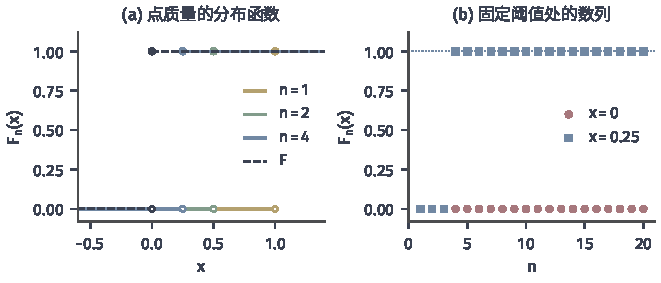
\includegraphics[width=112mm]{figures/02-abstract-mathematics/02-probability-spaces/matplotlib/wlim-point-mass-cdf/figure.pdf}
  \caption{点质量$\delta_{1/n}$的分布函数。(a) $n=1,2,4$时的$F_n$（实线）与极限$\delta_0$的分布函数$F$（虚线），实心点表示跳跃处取上方的值，空心点表示该处不取的值。(b) 固定阈值$x=0$与$x=0.25$时数列$F_n(x)$的取值，点线是$F(x)$。$x=0.25$处从$n=4$起$F_n(x)=1$；$x=0$处$F_n(0)$始终为$0$，而$F(0)=1$。}
  \label{fig:wlim-point-mass-cdf}
\end{figure}

\paragraph{连续点上的分布收敛}
例~\ref{ex:wlim-moving-point-mass}提示我们，只应在极限分布函数的连续点上要求收敛。

\begin{definition}[依分布收敛]
\label{def:wlim-convergence-in-distribution}
设$F_n$与$F$是实轴上的分布函数。若对$F$的每个连续点$x$都有$F_n(x)\to F(x)$，则称$F_n$\term{依分布收敛}（convergence in distribution）到$F$。
对分布函数分别为$F_n$和$F$的实值随机变量，同样称$X_n$依分布收敛到$X$，记作$X_n\Rightarrow X$。
\end{definition}

被排除的点不多。$F$单调不减，每个跳跃点$x$对应纵轴上的一个开区间$(F(x-),F(x))$，不同跳跃点的区间互不相交。
每个区间都含有理数，所以跳跃点至多可数，连续点在实轴上稠密。
极限因此是唯一的：若$F_n$同时依分布收敛到$F$和$G$，则$F$与$G$在两者公共连续点上相等，这些点仍然稠密；再由右连续性，从右侧逼近任一点即得$F=G$。

\paragraph{收敛的是分布而不是变量}
定义~\ref{def:wlim-convergence-in-distribution}只用到各个$X_n$的分布。
$X_n$可以定义在各自的概率空间$(\Omega_n,\mathcal F_n,\mathbb P_n)$上，$X$也可以换成任何与它同分布的随机变量，结论不受影响。
所以$X_n\Rightarrow X$实际是关于分布列$P_{X_n}$与分布$P_X$的陈述，它不要求这些变量共同实现，也不涉及$X_n$与$X$之间的差。
章首的模拟研究正是这种情形：每个$n$的数据单独生成，“$T_n$依分布趋近$N(0,1)$”有意义，“$T_n-Z$很小”却连定义都没有。

\subsection{度量空间上的弱收敛}

\paragraph{用有界连续函数检验}
分布函数依赖实数的大小顺序。随机向量、随机序列或随机函数的取值空间没有这样的顺序，我们需要一种不依赖顺序的比较方式。
自然的想法是挑选一类测试函数$h$，比较积分$\int h\,dP_n$与$\int h\,dP$。
事件的示性函数不适合做测试：例~\ref{ex:wlim-moving-point-mass}中$\delta_{1/n}(\{0\})=0$，而$\delta_0(\{0\})=1$，质量的微小移动就让它跳变。
连续函数则不会因微小移动而跳变。下面设$S$是度量空间，配以Borel $\sigma$代数，记$C_b(S)$为$S$上全体有界连续实值函数。

\begin{definition}[弱收敛]
\label{def:wlim-weak}
设$P_n$与$P$是度量空间$S$上的Borel概率测度。若对每个$h\in C_b(S)$都有
\[
  \int_S h\,dP_n\to\int_S h\,dP,
\]
则称$P_n$\term{弱收敛}（weak convergence）到$P$，记作$P_n\Rightarrow P$。
对取值于$S$的随机对象，若$P_{X_n}\Rightarrow P_X$，也称$X_n$依分布收敛到$X$，记作$X_n\Rightarrow X$。
\end{definition}

有界性保证每个测试积分有限；连续性保证取值的微小移动只引起测试值的微小变化。
由定理~\ref{thm:pmod-change-of-variables}，$\int h\,dP_{X_n}=\mathbb E\,h(X_n)$，所以随机对象的条件可以写成：对每个$h\in C_b(S)$，$\mathbb E\,h(X_n)\to\mathbb E\,h(X)$，其中各个期望分别在$X_n$与$X$所在的概率空间上计算。
回到移动的点质量，$\int h\,d\delta_{1/n}=h(1/n)\to h(0)$，所以$\delta_{1/n}\Rightarrow\delta_0$。
这里只使用一类测试函数，不需要在测度集合上另外构造范数或拓扑结构。

\paragraph{闭集的连续逼近与极限的唯一性}
连续测试函数虽然不能直接取成示性函数，却能从上方逼近闭集的示性函数。
这一构造既用来说明弱极限唯一，也是下文开闭集判据的出发点。

\begin{lemma}[闭集的距离逼近]
\label{lem:wlim-closed-approximation}
设$F$是度量空间$S$中的非空闭集，$d(x,F)=\inf_{y\in F}d(x,y)$。对正整数$k$令
\[
  h_k(x)=\max\{0,\,1-k\,d(x,F)\}.
\]
则每个$h_k$连续且$0\leq h_k\leq1$，在$F$上等于$1$；并且对每个$x\in S$，$h_k(x)$随$k$单调不增地趋于$\mathbb I_F(x)$。
\end{lemma}

\begin{proof}
由三角不等式，$|d(x,F)-d(y,F)|\leq d(x,y)$，所以$x\mapsto d(x,F)$连续，$h_k$连续且取值在$[0,1]$中。
若$x\in F$，则$d(x,F)=0$，$h_k(x)=1$。若$x\notin F$，因$F$闭，存在以$x$为中心的球与$F$不交，故$d(x,F)>0$；当$k>1/d(x,F)$时$h_k(x)=0$。$h_k$关于$k$单调不增是因为$1-k\,d(x,F)$关于$k$不增。
\end{proof}

\begin{lemma}[弱极限的唯一性]
\label{lem:wlim-uniqueness-limit}
设$P,Q$是度量空间$S$上的Borel概率测度。若对每个$h\in C_b(S)$都有$\int h\,dP=\int h\,dQ$，则$P=Q$。特别地，若$P_n\Rightarrow P$且$P_n\Rightarrow Q$，则$P=Q$。
\end{lemma}

\begin{proof}
对非空闭集$F$取引理~\ref{lem:wlim-closed-approximation}中的$h_k$。$h_k\to\mathbb I_F$逐点成立且$|h_k|\leq1$，由控制收敛定理，$P(F)=\lim_k\int h_k\,dP=\lim_k\int h_k\,dQ=Q(F)$；空集上两者都为零。
闭集族对有限交封闭，并且生成Borel $\sigma$代数，由定理~\ref{thm:measure-pi-lambda-uniqueness}得$P=Q$。
若$P_n$同时弱收敛到$P$和$Q$，则$\int h\,dP$与$\int h\,dQ$都是同一数列$\int h\,dP_n$的极限，从而相等。
\end{proof}

图~\ref{fig:wlim-closed-set-portmanteau}(a)以闭区间$F=[-1,0]$为例画出$h_k$：它们是一族梯形，平顶覆盖$F$，两侧斜坡宽度为$1/k$，随$k$增大而收窄，从上方压向$F$的示性函数。

\begin{figure}[htbp]
  \centering
  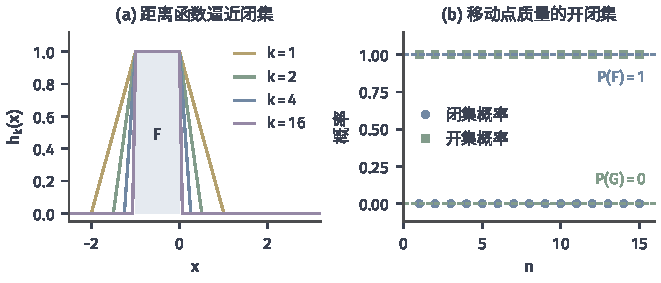
\includegraphics[width=112mm]{figures/02-abstract-mathematics/02-probability-spaces/matplotlib/wlim-closed-set-portmanteau/figure.pdf}
  \caption{闭集的连续逼近与开闭集上的概率界。(a) 闭集$F=[-1,0]$（浅蓝区域）的距离逼近$h_k(x)=\max\{0,1-k\,d(x,F)\}$，$k=1,2,4,16$。(b) 对$P_n=\delta_{1/n}$与$P=\delta_0$，圆点是闭集$F=(-\infty,0]$的概率$P_n(F)=0$，方点是开集$G=(0,\infty)$的概率$P_n(G)=1$，虚线分别是极限测度的概率$P(F)=1$与$P(G)=0$。}
  \label{fig:wlim-closed-set-portmanteau}
\end{figure}

\paragraph{与分布函数判据的等价}
在实轴上我们现在有两种定义：分布函数在连续点收敛，以及有界连续函数的积分收敛。
下面的定理说明二者一致，因此本章此后不再区分“依分布收敛”与“弱收敛”所指的分布趋近。

\begin{theorem}[实轴上两种定义的等价]
\label{thm:wlim-real-equivalence}
设$P_n,P$是$\mathbb R$上的Borel概率测度，分布函数分别为$F_n,F$。则$P_n\Rightarrow P$当且仅当$F$的每个连续点$x$处都有$F_n(x)\to F(x)$。
\end{theorem}

\begin{proof}
先证弱收敛推出分布函数收敛。固定$F$的连续点$x$和$\delta>0$，令$h_+$在$(-\infty,x]$上等于$1$、在$[x+\delta,\infty)$上等于$0$、中间线性下降；令$h_-$在$(-\infty,x-\delta]$上等于$1$、在$[x,\infty)$上等于$0$、中间线性下降。
两者都有界连续，并且$h_-\leq\mathbb I_{(-\infty,x]}\leq h_+$。对$P_n$积分得$\int h_-\,dP_n\leq F_n(x)\leq\int h_+\,dP_n$，令$n\to\infty$，
\[
  \begin{aligned}
  F(x-\delta)&\leq\int h_-\,dP\leq\liminf_nF_n(x)\\
  &\leq\limsup_nF_n(x)\leq\int h_+\,dP\leq F(x+\delta).
  \end{aligned}
\]
两端的不等式来自$\mathbb I_{(-\infty,x-\delta]}\leq h_-$与$h_+\leq\mathbb I_{(-\infty,x+\delta]}$。令$\delta\downarrow0$，由$F$在$x$处连续，两端都趋于$F(x)$。

再证反方向。设$h\in C_b(\mathbb R)$，$|h|\leq M$，固定$\varepsilon\in(0,1)$。
由于$F$的连续点稠密且$F(-\infty)=0$、$F(\infty)=1$，可取$F$的连续点$a<b$使$F(a)<\varepsilon$、$1-F(b)<\varepsilon$。
$h$在紧区间$[a,b]$上一致连续（定理~\ref{thm:metric-heine-cantor}），取$\eta>0$使$|x-y|\leq\eta$时$|h(x)-h(y)|<\varepsilon$；再取$F$的连续点$a=x_0<x_1<\dots<x_m=b$，相邻间距不超过$\eta$。
令$g=\sum_{j=1}^mh(x_j)\mathbb I_{(x_{j-1},x_j]}$，则在$(a,b]$上$|h-g|<\varepsilon$，在$(a,b]$外$g=0$。于是对$Q=P_n$或$Q=P$都有
\[
  \Bigl|\int h\,dQ-\int g\,dQ\Bigr|\leq\varepsilon+M\,Q\bigl(\mathbb R\setminus(a,b]\bigr).
\]
又$\int g\,dP_n=\sum_jh(x_j)\bigl(F_n(x_j)-F_n(x_{j-1})\bigr)\to\int g\,dP$，且$P_n(\mathbb R\setminus(a,b])=F_n(a)+1-F_n(b)\to F(a)+1-F(b)<2\varepsilon$。
合并得$\limsup_n|\int h\,dP_n-\int h\,dP|\leq2\varepsilon+4M\varepsilon$，而$\varepsilon$任意。
\end{proof}

图~\ref{fig:wlim-halfline-sandwich}展示了正向证明的两个动作：(a)中两条连续斜坡从两侧夹住半直线的示性函数；(b)以标准正态分布函数为例，上下界$F(x+\delta)$与$F(x-\delta)$随$\delta\to0$收拢到$F(x)$，这一步正是连续点条件发挥作用的地方。
反向证明把实轴分成紧区间和两端尾部分别处理，这样的分割不能省去：$h(x)=\sin(x^2)$有界连续，但在整条实轴上不一致连续，不能用一个统一的阶梯函数逼近；尾部只能依靠概率质量小来控制。

\begin{figure}[htbp]
  \centering
  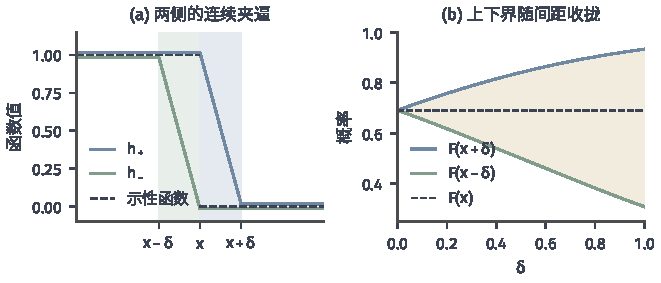
\includegraphics[width=112mm]{figures/02-abstract-mathematics/02-probability-spaces/matplotlib/wlim-halfline-sandwich/figure.pdf}
  \caption{用连续函数夹住半直线的示性函数。(a) 阈值$x=0$、间距$\delta=0.5$时的斜坡函数$h_-\leq\mathbb I_{(-\infty,x]}\leq h_+$，两条曲线略作上下错开以便区分。(b) 取$F$为标准正态分布函数、$x=0.5$，上界$F(x+\delta)$与下界$F(x-\delta)$随$\delta$减小收拢到$F(0.5)\approx0.691$（虚线）。}
  \label{fig:wlim-halfline-sandwich}
\end{figure}

\subsection{与依概率收敛的关系}

\paragraph{依概率收敛推出分布收敛}
当$X_n$与$X$定义在同一概率空间上时，第~\ref{chap:random-variable-convergence}章的依概率收敛（定义~\ref{def:conv-probability}）要求对每个$\varepsilon>0$都有$\mathbb P(\lVert X_n-X\rVert>\varepsilon)\to0$。
它比较的是逐样本误差，自然应当比只比较分布的弱收敛更强。证明用到该章的子列判据（定理~\ref{thm:conv-subsequence}）：$X_n\xrightarrow{\mathbb P}X$当且仅当每个子列都有进一步的子列几乎必然收敛到$X$。

\begin{theorem}[依概率收敛推出依分布收敛]
\label{thm:wlim-probability-implies-distribution}
设$\bm X_n,\bm X$是同一概率空间上的$\mathbb R^d$值随机向量。若$\bm X_n\xrightarrow{\mathbb P}\bm X$，则$\bm X_n\Rightarrow\bm X$。
\end{theorem}

\begin{proof}
设$h\in C_b(\mathbb R^d)$，$|h|\leq M$。若$\mathbb E\,h(\bm X_n)\not\to\mathbb E\,h(\bm X)$，则存在$\varepsilon>0$及子列$n_k$，使$|\mathbb E\,h(\bm X_{n_k})-\mathbb E\,h(\bm X)|\geq\varepsilon$对所有$k$成立。
由子列判据，$n_k$中还有子列$n_{k_j}$使$\bm X_{n_{k_j}}\to\bm X$几乎必然成立；$h$连续，故$h(\bm X_{n_{k_j}})\to h(\bm X)$几乎必然成立。
这些变量都以常数$M$为界，由控制收敛定理得$\mathbb E\,h(\bm X_{n_{k_j}})\to\mathbb E\,h(\bm X)$，与上面的不等式矛盾。
\end{proof}

同一论证适用于可分度量空间上的随机对象，这里不需要完备性。在可分的取值空间中$d(X_n,X)$是随机变量，依概率收敛定义为对每个$\varepsilon>0$都有$\mathbb P(d(X_n,X)>\varepsilon)\to0$；对实值变量$d(X_n,X)$使用子列判据，再重复上面的控制收敛论证，即得$X_n\Rightarrow X$。

\paragraph{向常数的分布收敛}
反方向一般不成立，但极限是常数时成立。此时依概率收敛只涉及$X_n$自身偏离常数$\bm c$的概率，不需要共同的极限变量。

\begin{theorem}[向常数的分布收敛]
\label{thm:wlim-constant-limit}
设$\bm X_n$是$\mathbb R^d$值随机向量（可以定义在不同概率空间上），$\bm c\in\mathbb R^d$为常向量。若$\bm X_n\Rightarrow\delta_{\bm c}$，则对每个$\varepsilon>0$都有$\mathbb P(\lVert\bm X_n-\bm c\rVert\geq\varepsilon)\to0$。
\end{theorem}

\begin{proof}
令$h(\bm x)=\min\{1,\lVert\bm x-\bm c\rVert/\varepsilon\}$，它有界连续，$h(\bm c)=0$，并且在$\{\lVert\bm x-\bm c\rVert\geq\varepsilon\}$上等于$1$。于是
\[
  \mathbb P(\lVert\bm X_n-\bm c\rVert\geq\varepsilon)\leq\mathbb E\,h(\bm X_n)\to h(\bm c)=0.
\]
不等式成立是因为$h$非负且在事件$\{\lVert\bm X_n-\bm c\rVert\geq\varepsilon\}$上等于$1$，极限来自依分布收敛的定义。
\end{proof}

当各个$\bm X_n$定义在不同概率空间上时，上式左端在各自的空间中计算，“$\bm X_n$依概率收敛到常数$\bm c$”仍然有意义，后文的Slutsky规则会用到这种形式。
与定理~\ref{thm:wlim-probability-implies-distribution}合起来，向常数的依分布收敛与依概率收敛等价。

\paragraph{同分布序列未必依概率收敛}
极限不是常数时，弱收敛不能推出依概率收敛。第~\ref{chap:probability-models}章的例~\ref{ex:pmod-alternating-bits}已经用交替序列说明，同分布的随机变量可以在样本点上相距很远；这里把它改写成符号形式，检验收敛方式的逆向关系。

\begin{example}[交替符号序列]
\label{ex:wlim-alternating-sign}
设$Z$以相等概率取$\pm1$，令$X_n=(-1)^nZ$。$-Z$与$Z$同分布，所以每个$X_n$都与$Z$同分布，$X_n\Rightarrow Z$平凡成立。
但当$n$为奇数时，$|X_n-Z|=2|Z|=2$恒成立，$\mathbb P(|X_n-Z|>1)=1$，所以$X_n$不依概率收敛到$Z$。
事实上$X_n$不依概率收敛到任何随机变量：偶数项恒等于$Z$，奇数项恒等于$-Z$，两个子列的极限不同。
\end{example}

弱收敛只记录各个$X_n$的分布，不记录$X_n$与$Z$在同一样本点上怎样配对；例~\ref{ex:wlim-alternating-sign}中分布始终不变，配对却在同号与反号之间交替。第~\ref{sec:wlim-joint-transform}节会看到，这种配对信息正是联合分布要补充的内容。

\subsection{开闭集与连续集上的概率}

\paragraph{开闭集上的概率界}
弱收敛用函数积分定义，但我们常常关心事件概率$P_n(A)$是否趋于$P(A)$。
移动的点质量说明不能对所有事件期望这一点：如图~\ref{fig:wlim-closed-set-portmanteau}(b)所示，对闭集$F=(-\infty,0]$有$P_n(F)=0<1=P(F)$，对开集$G=(0,\infty)$有$P_n(G)=1>0=P(G)$。
这里的质量原本在开集$G$内部，极限时落到$G$的边界点$0$上，而$0$属于闭集$F$。
质量落到边界上，可以让极限测度给闭集更多概率、给开集更少概率；反方向的跳变却不会发生。下面的定理把这一观察变成等价判据。

\begin{theorem}[\term{Portmanteau定理}]
\label{thm:wlim-portmanteau}
设$P_n,P$是度量空间$S$上的Borel概率测度。以下四条等价：
\begin{enumerate}
  \item $P_n\Rightarrow P$；
  \item 对每个闭集$F$，$\limsup_nP_n(F)\leq P(F)$；
  \item 对每个开集$G$，$\liminf_nP_n(G)\geq P(G)$；
  \item 对每个满足$P(\partial A)=0$的Borel集$A$，$P_n(A)\to P(A)$。
\end{enumerate}
\end{theorem}

\begin{proof}
由(1)推(2)。$F$为空集时结论平凡。对非空闭集$F$取引理~\ref{lem:wlim-closed-approximation}的$h_k$。由$\mathbb I_F\leq h_k$，
\[
  \limsup_nP_n(F)\leq\lim_n\int h_k\,dP_n=\int h_k\,dP.
\]
令$k\to\infty$，由控制收敛定理右端趋于$P(F)$。

(2)与(3)等价，因为开集的补集是闭集，而$P_n(G)=1-P_n(S\setminus G)$。

由(2)(3)推(4)。记$A^\circ$与$\overline A$为$A$的内部和闭包，$\partial A=\overline A\setminus A^\circ$。由$P(\partial A)=0$得$P(A^\circ)=P(A)=P(\overline A)$，于是
\[
  \begin{aligned}
  \limsup_nP_n(A)&\leq\limsup_nP_n(\overline A)\leq P(\overline A)=P(A),\\
  \liminf_nP_n(A)&\geq\liminf_nP_n(A^\circ)\geq P(A^\circ)=P(A).
  \end{aligned}
\]

由(4)推(1)。设$h\in C_b(S)$。对$h$作正仿射变换不改变结论，故不妨设$0<h<1$。由Tonelli定理（定理~\ref{thm:analysis-tonelli-fubini}），对任一概率测度$Q$，
\[
  \int h\,dQ=\int_S\int_0^1\mathbb I_{\{t<h(x)\}}\,dt\,Q(dx)=\int_0^1Q(h>t)\,dt.
\]
$h$连续，所以$\{h>t\}$是开集、$\{h\geq t\}$是闭集，边界含于$\{h=t\}$。集合$\{h=t\}$对不同$t$互不相交，其中$P$概率为正的至多可数个，因此除可数个$t$外都有$P(h=t)=0$，从而$P_n(h>t)\to P(h>t)$。
被积函数以$1$为界，对$dt$在$[0,1]$上使用控制收敛定理，即得$\int h\,dP_n\to\int h\,dP$。
\end{proof}

定理的(2)(3)是单向的：闭集的概率在极限处只可能增加，开集的概率只可能减少，因为质量可以从开集内部移到边界上，而边界属于相应的闭集。
证明的最后一步用水平集$\{h>t\}$把一个连续测试函数分解成一族开集，这是从事件概率回到积分的通用桥梁。

\paragraph{边界零质量的集合}
定理~\ref{thm:wlim-portmanteau}的(4)给出一类保证概率收敛的事件：满足$P(\partial A)=0$的Borel集合称为$P$的\term{连续集}（continuity set）。
在实轴上取$A=(-\infty,x]$，其边界是$\{x\}$，$P(\{x\})=F(x)-F(x-)$，所以$A$是连续集恰好等价于$x$是$F$的连续点。
定义~\ref{def:wlim-convergence-in-distribution}中“只在连续点要求收敛”的规定，因而是一般边界零质量条件在半直线上的特例。

边界零质量是充分条件而不是必要条件。若$P_n=P=\delta_0$对所有$n$成立，取$A=\{0\}$，则$P(\partial A)=1$，而$P_n(A)=P(A)$对所有$n$都成立。
条件说明的是：只要边界上没有极限质量，质量在边界两侧的移动就不影响概率的极限；边界上有质量时，需要另外检查质量从哪一侧趋近。

\subsection{分布积分的极限}

\paragraph{无界函数的积分}
弱收敛的定义已经保证有界连续函数的积分收敛。可是均值、方差等矩来自无界函数$x$、$x^2$，定义本身不覆盖它们。
第~\ref{chap:random-variable-convergence}章的尖峰变量（例~\ref{ex:conv-spike}）说明这里确有缺口：$U\sim\mathrm{Unif}[0,1)$，$X_n=n\mathbb I_{(0,1/n)}(U)$以概率$1/n$取$n$、其余时候取$0$。
那里关心$X_n$在样本点上趋于零而期望恒为$1$；这里只看它们的分布。

\begin{example}[尖峰分布]
\label{ex:wlim-spike-distribution}
令$P_n=(1-1/n)\delta_0+(1/n)\delta_n$，即上述$X_n$的分布。对$h\in C_b(\mathbb R)$，$|h|\leq M$，
\[
  \int h\,dP_n=\Bigl(1-\frac1n\Bigr)h(0)+\frac1nh(n)\to h(0),
\]
因为$|h(n)|/n\leq M/n\to0$。所以$P_n\Rightarrow\delta_0$。但对每个$n$都有$\int x\,P_n(dx)=1$，而极限的均值是$0$。
\end{example}

图~\ref{fig:wlim-spike-mean}(a)画出$n=10$与$n=40$的尖峰分布：远处的点质量越来越小，却越来越远，二者乘积保持为$1$。
(b)比较均值与截断均值$\int\min\{x,M\}\,dP_n=\min\{n,M\}/n$：截断函数$\min\{x,M\}$在分布的支撑$[0,\infty)$上有界连续，它的积分随$n$增大趋于零，符合弱收敛；不截断的均值则停在$1$。
差别完全来自尾部：远处很小的质量乘上很大的函数值，仍贡献了不消失的积分。

\begin{figure}[htbp]
  \centering
  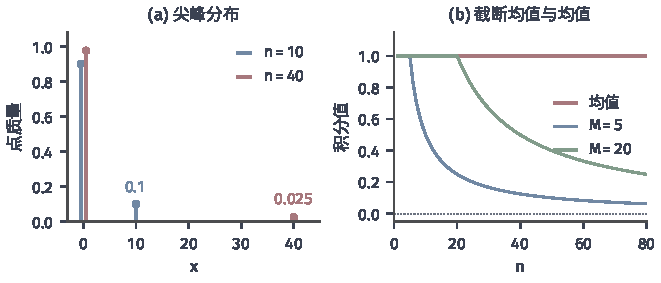
\includegraphics[width=112mm]{figures/02-abstract-mathematics/02-probability-spaces/matplotlib/wlim-spike-mean/figure.pdf}
  \caption{弱收敛但均值不收敛的尖峰分布$P_n=(1-1/n)\delta_0+(1/n)\delta_n$。(a) $n=10$与$n=40$时的点质量，原点处的两根竖线略作左右错开。(b) 均值$\int x\,dP_n=1$与截断均值$\int\min\{x,M\}\,dP_n=\min\{n,M\}/n$（$M=5,20$）随$n$的变化。}
  \label{fig:wlim-spike-mean}
\end{figure}

\paragraph{沿分布列的一致可积}
第~\ref{chap:random-variable-convergence}章用一致可积（定义~\ref{def:conv-uniform-integrability}）控制同一概率空间上随机变量的尾部积分。只看分布时，同样的尾部条件可以直接写在分布列上。

\begin{definition}[沿分布列的一致可积]
\label{def:wlim-ui-sequence}
设$P_n$是度量空间$S$上的Borel概率测度，$h:S\to\mathbb R$连续。若
\[
  \lim_{M\to\infty}\sup_n\int|h|\,\mathbb I_{\{|h|>M\}}\,dP_n=0,
\]
则称$h$关于$\{P_n\}$一致可积。
\end{definition}

若$X_n$的分布是$P_n$，这正是随机变量族$\{h(X_n)\}$的一致可积性；不同的是各个$X_n$可以定义在不同概率空间上。
尖峰分布不满足这一条件：取$h(x)=x$，当$n>M$时$\int|x|\,\mathbb I_{\{|x|>M\}}\,dP_n=1$。

\begin{theorem}[一致可积下的积分极限]
\label{thm:wlim-ui-integral}
设$P_n\Rightarrow P$，$h:S\to\mathbb R$连续且关于$\{P_n\}$一致可积。则$h$关于$P$可积，并且$\int h\,dP_n\to\int h\,dP$。
\end{theorem}

\begin{proof}
记$\tau(M)=\sup_n\int|h|\,\mathbb I_{\{|h|>M\}}\,dP_n$。

第一步，极限测度下的可积性。取$M_0$使$\tau(M_0)\leq1$，则
\[
  \sup_n\int|h|\,dP_n\leq M_0+1.
\]
对每个$L>0$，函数$\min\{|h|,L\}$有界连续，因此
\[
  \int\min\{|h|,L\}\,dP=\lim_n\int\min\{|h|,L\}\,dP_n\leq M_0+1.
\]
令$L\to\infty$，由单调收敛定理得$\int|h|\,dP\leq M_0+1$。于是$|h|\,\mathbb I_{\{|h|>M\}}\leq|h|$且逐点趋于零，由控制收敛定理，$\int|h|\,\mathbb I_{\{|h|>M\}}\,dP\to0$。

第二步，截断。令$h_M=\max\{-M,\min\{h,M\}\}$，它有界连续，并且$|h-h_M|\leq|h|\,\mathbb I_{\{|h|>M\}}$。于是
\[
  \Bigl|\int h\,dP_n-\int h\,dP\Bigr|\leq\tau(M)+\Bigl|\int h_M\,dP_n-\int h_M\,dP\Bigr|+\int|h|\,\mathbb I_{\{|h|>M\}}\,dP.
\]
先令$n\to\infty$，中间一项趋于零；再令$M\to\infty$，其余两项趋于零。
\end{proof}

证明的两次极限顺序不能交换：截断阈值$M$固定时，弱收敛处理有界部分；一致可积保证尾部误差对所有$n$同时小，才允许最后令$M\to\infty$。
尖峰分布在第二步失效：取$h(x)=x$时，对每个$M$都有$\tau(M)=1$，尾部误差不随$M$增大而减小。

\paragraph{均值与矩的收敛}
在$\mathbb R^d$上，最常用的无界函数是坐标$x_j$、乘积$x_ix_j$与范数的幂$\lVert\bm x\rVert^p$。下面给出一个易于检验的充分条件。

\begin{theorem}[矩的收敛]
\label{thm:wlim-moment-convergence}
设$\mathbb R^d$上的概率测度$P_n\Rightarrow P$，并且对某个$p>0$与$\delta>0$，
\[
  K=\sup_n\int\lVert\bm x\rVert^{p+\delta}\,P_n(d\bm x)<\infty.
\]
则对每个满足$|h(\bm x)|\leq C(1+\lVert\bm x\rVert^p)$的连续函数$h$，都有$\int h\,dP_n\to\int h\,dP$。
特别地，$p\geq1$时各坐标的均值收敛，$p\geq2$时二阶矩与协方差收敛。
\end{theorem}

\begin{proof}
令$r=(p+\delta)/p>1$。在$\{|h|>M\}$上$|h|=|h|^r|h|^{1-r}\leq|h|^rM^{1-r}$，并且由$(a+b)^r\leq2^{r-1}(a^r+b^r)$，
\[
  |h|^r\leq C^r2^{r-1}\bigl(1+\lVert\bm x\rVert^{p+\delta}\bigr).
\]
因此$\sup_n\int|h|\,\mathbb I_{\{|h|>M\}}\,dP_n\leq M^{1-r}C^r2^{r-1}(1+K)\to0$，再用定理~\ref{thm:wlim-ui-integral}。
坐标满足$|x_j|\leq\lVert\bm x\rVert\leq1+\lVert\bm x\rVert^p$（$p\geq1$），乘积满足$|x_ix_j|\leq\lVert\bm x\rVert^2\leq1+\lVert\bm x\rVert^p$（$p\geq2$），于是均值与二阶矩收敛，协方差由它们组合而成。
\end{proof}

这个条件要求略高于$p$阶的矩一致有界，仅有$p$阶矩一致有界还不够：尖峰分布的一阶矩恒为$1$，均值却不收敛到极限分布的均值；它的$1+\delta$阶矩等于$n^\delta$，确实没有一致上界。
把弱收敛与矩控制合成一种更强的分布距离，并用于比较分布和优化问题，是\BookPartRef{part:probability-distributions}{卷四“概率分布”部分}的任务。

\section{概率分布族的紧性}
\label{sec:wlim-tightness}

上一节总是先有候选极限$P$，再检验$P_n$是否趋近它。中心极限定理一类问题的困难恰在于极限需要被找出来。
本节先不指定极限，研究一族概率分布能否抽出弱收敛子列：先区分单个分布与整族分布的质量控制，再给出判别条件和子列存在定理，最后说明怎样从子列回到整列。

\subsection{紧性与一致紧性}

\paragraph{质量留在紧集中}
实数列有界时总有收敛子列，有界性阻止了数列跑向无穷远。
对概率分布列，相应的危险是概率质量跑出任何固定范围，例如$\delta_n$的全部质量随$n$移向无穷远，在极限中不留下任何东西。
第~\ref{chap:metric-spaces}章的紧集是度量空间中“既有界又不漏点”的范围，我们用它来约束质量的位置。

\begin{definition}[紧性与一致紧性]
\label{def:wlim-tight}
设$S$是度量空间。若对每个$\varepsilon>0$都存在紧集$K\subseteq S$使$P(K)>1-\varepsilon$，则称Borel概率测度$P$是紧的。
若对每个$\varepsilon>0$都存在\emph{同一个}紧集$K$，使族$\Pi$中每个$P$都满足$P(K)>1-\varepsilon$，则称概率族$\Pi$一致紧（uniformly tight），这一性质称为\term{一致紧性}。
\end{definition}

两者的差别在量词次序。紧性是“对每个$P$，存在$K$”，紧集可以随$P$改变；一致紧性是“存在$K$，对每个$P$”，紧集只能随精度$\varepsilon$改变，不能随族中成员改变。
一致紧性约束的是概率质量所在的范围，不约束质量在这个范围内怎样分布。

\paragraph{Polish空间上的单个分布}
在常用的取值空间中，单个概率测度总是紧的。所需的空间条件是：度量空间完备，并且有可数稠密子集，这样的空间称为\term{Polish空间}（Polish space）。$\mathbb R^d$、可数集配以离散度量，以及后续部分中的许多序列和函数空间都属于此类。

\begin{theorem}[Polish空间上的概率测度是紧的]
\label{thm:wlim-polish-tight}
设$S$是Polish空间，则$S$上每个Borel概率测度$P$都是紧的。
\end{theorem}

\begin{proof}
取$S$的可数稠密子集$\{s_1,s_2,\ldots\}$，固定$\varepsilon>0$。对每个正整数$m$，闭球$\overline B(s_j,1/m)$（$j\geq1$）覆盖$S$；由概率测度的下连续性，存在$N_m$使
\[
  P\Bigl(\bigcup_{j\leq N_m}\overline B(s_j,1/m)\Bigr)>1-\varepsilon2^{-m}.
\]
令$K=\bigcap_{m\geq1}\bigcup_{j\leq N_m}\overline B(s_j,1/m)$。$K$是闭集的交，因而闭；对每个$m$，$K$被有限个半径$1/m$的闭球覆盖，因而全有界。
完备空间的闭子集完备，由定理~\ref{thm:metric-complete-totally-bounded}，$K$紧。最后$P(S\setminus K)\leq\sum_m\varepsilon2^{-m}=\varepsilon$。
\end{proof}

证明用到三个结构：可分性提供可数个球心，概率的下连续性把无限覆盖截成有限覆盖，完备性保证有限覆盖的交确实是紧集。

\paragraph{逐个紧不推出一致紧}
定理~\ref{thm:wlim-polish-tight}只说明每个分布单独是紧的。点质量族$\{\delta_n:n\geq1\}$说明这不能推出一致紧：每个$\delta_n$的全部质量在单点$\{n\}$上，单点是紧集；但实轴上任何紧集$K$都有界，含于某个$[-R,R]$，当$n>R$时$\delta_n(K)=0$。

图~\ref{fig:wlim-escape-tight}(a)用“族内最大外部概率”$R\mapsto\sup_nP_n(|x|>R)$比较三族分布，一致紧性等价于这条曲线随$R\to\infty$趋于零。
$\{\delta_n\}$的曲线恒为$1$。尖峰分布族的曲线是$1/(\lfloor R\rfloor+1)$，趋于零，所以尖峰分布族一致紧，尽管它的均值不收敛到极限分布的均值；这说明一致紧性与上一节的一致可积控制的是不同的东西。
方差在$(1,2]$中的正态族由方差最大的成员控制，曲线是$\mathbb P(|N(0,2)|>R)$。图(b)把$\delta_n$的位置与一个固定窗口$[-R,R]$放在一起，窗口之外的点质量不断出现。

\begin{figure}[htbp]
  \centering
  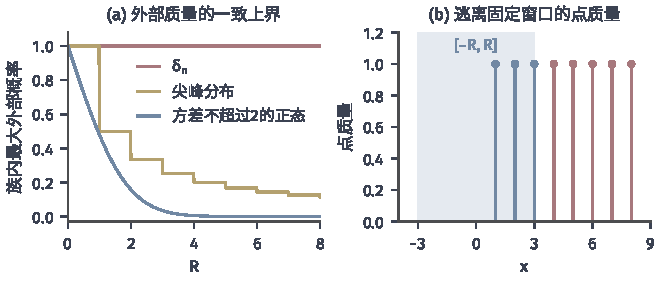
\includegraphics[width=112mm]{figures/02-abstract-mathematics/02-probability-spaces/matplotlib/wlim-escape-tight/figure.pdf}
  \caption{逃逸的点质量与一致紧的分布族。(a) 族内最大外部概率$\sup_nP_n(|x|>R)$：$\{\delta_n\}$恒为$1$；尖峰分布族$\{(1-1/n)\delta_0+(1/n)\delta_n\}$为$1/(\lfloor R\rfloor+1)$；正态族$\{N(0,1+1/n)\}$为$\mathbb P(|N(0,2)|>R)$。(b) 点质量$\delta_1,\ldots,\delta_8$与窗口$[-3,3]$（浅蓝区域），窗口外的点质量以红色标出。}
  \label{fig:wlim-escape-tight}
\end{figure}

\subsection{一致紧性的判别}

\paragraph{矩的一致上界}
在$\mathbb R^d$中，有界闭集紧（Heine--Borel判据），所以一致紧性就是大球外概率对全族一致消失：对每个$\varepsilon>0$存在$R$，使$\sup_nP_n(\lVert\bm x\rVert>R)<\varepsilon$。
Markov不等式（定理~\ref{thm:pmod-markov}）把这种尾部概率交给矩来控制。

\begin{theorem}[矩上界推出一致紧]
\label{thm:wlim-moment-tightness}
设$P_n$是$\mathbb R^d$上的概率测度。若对某个$p>0$有$C=\sup_n\int\lVert\bm x\rVert^p\,P_n(d\bm x)<\infty$，则$\{P_n\}$一致紧。
\end{theorem}

\begin{proof}
闭球$\overline B(\bm 0,R)$紧，并且由Markov不等式，$P_n(\lVert\bm x\rVert>R)\leq C/R^p$对所有$n$成立。取$R$使$C/R^p<\varepsilon$即可。
\end{proof}

定理要求的是矩的统一上界，逐项有限不够：$\delta_n$的每阶矩都有限，但$\int|x|^p\,d\delta_n=n^p$没有统一上界。
定理也只提供取得弱极限子列所需的质量控制，不说明整列收敛，更不说明同阶矩收敛：尖峰分布满足$\sup_n\int|x|\,dP_n=1$，因而一致紧，但均值不收敛到极限分布的均值。

另一个常用的一致紧来源是弱收敛本身。

\begin{lemma}[弱收敛列一致紧]
\label{lem:wlim-convergent-tight}
设$\mathbb R^d$上的概率测度$P_n\Rightarrow P$，则$\{P_n\}$一致紧。
\end{lemma}

\begin{proof}
固定$\varepsilon>0$，取$R$使$P(\lVert\bm x\rVert\geq R)<\varepsilon$。集合$\{\lVert\bm x\rVert\geq R\}$是闭集，由定理~\ref{thm:wlim-portmanteau}，$\limsup_nP_n(\lVert\bm x\rVert\geq R)\leq P(\lVert\bm x\rVert\geq R)<\varepsilon$，所以存在$N$使$n\geq N$时$P_n(\lVert\bm x\rVert\geq R)<\varepsilon$。
前$N-1$个测度各自是紧的：对单个概率测度$P_n$，$P_n(\lVert\bm x\rVert\geq r)\to0$（$r\to\infty$），所以各自存在使外部概率小于$\varepsilon$的半径。把$R$增大到这些半径的最大值，紧集$\overline B(\bm 0,R)$即对全族适用。
\end{proof}

\paragraph{紧次水平集}
定理~\ref{thm:wlim-moment-tightness}的证明实际只用到一点：函数$\lVert\bm x\rVert^p$不超过给定水平的点构成紧集。这一结构可以推广到一般度量空间。

\begin{theorem}[紧次水平集的控制函数]
\label{thm:wlim-sublevel-tightness}
设$S$是度量空间，$V:S\to[0,\infty)$可测，并且对每个$R\geq0$，次水平集$\{V\leq R\}$紧。若$C=\sup_n\int V\,dP_n<\infty$，则$\{P_n\}$一致紧。
\end{theorem}

\begin{proof}
由Markov不等式，$P_n(V>R)\leq C/R$对所有$n$成立，而$\{V\leq R\}$是紧集。取$R>C/\varepsilon$即可。
\end{proof}

推广时起作用的是“次水平集紧”；只找到一个积分一致有界的函数并不够，因为在一般度量空间中有界闭集未必紧。例如在自然数集$\mathbb N$上取离散度量（不同点距离为$1$），它是Polish空间。
令$V(x)=d(x,0)\leq1$，则$\sup_n\int V\,d\delta_n\leq1$；但$\{V\leq1\}=\mathbb N$不紧，离散空间的紧集只能是有限集，$\{\delta_n\}$也不一致紧。

\subsection{弱收敛子列的存在}

\paragraph{有理点上的对角线选择}
现在在实轴上构造弱收敛子列。分布函数取值在$[0,1]$中，每个固定阈值处的数列都有收敛子列；困难在于阈值有不可数多个。
我们只在可数个有理点上取子列，再用单调性把极限延拓到整条实轴。

\begin{lemma}[\term{Helly选择定理}]
\label{lem:wlim-helly}
设$F_n$是实轴上的分布函数列。则存在子列$F_{n_k}$及单调不减、右连续、取值于$[0,1]$的函数$G$，使在$G$的每个连续点$x$处都有$F_{n_k}(x)\to G(x)$。
\end{lemma}

\begin{proof}
把有理数排成$q_1,q_2,\ldots$。数列$F_n(q_1)$在$[0,1]$中有界，有收敛子列；在这个子列中，$F_n(q_2)$又有收敛的子子列；如此依次取下去，得到一串嵌套的子列。取第$k$个子列中的第$k$项为$n_k$，则对每个$j$，$(n_k)_{k\geq j}$都是第$j$个子列的子列，于是$F_{n_k}(q)$对每个有理数$q$都收敛，记极限为$H(q)$。

$H$在有理数上单调不减。令$G(x)=\inf\{H(q):q\in\mathbb Q,\,q>x\}$，它单调不减。
若$x_m\downarrow x$，对每个有理数$q>x$，当$m$充分大时$x_m<q$，故$\lim_mG(x_m)\leq H(q)$；对$q$取下确界得$\lim_mG(x_m)\leq G(x)$，而单调性给出反向不等式，所以$G$右连续。

设$x$是$G$的连续点。对有理数$s>x$，$F_{n_k}(x)\leq F_{n_k}(s)\to H(s)$，对$s$取下确界得$\limsup_kF_{n_k}(x)\leq G(x)$。
对$y<x$取有理数$q\in(y,x)$，则$G(y)\leq H(q)$，而$H(q)=\lim_kF_{n_k}(q)\leq\liminf_kF_{n_k}(x)$；令$y\uparrow x$，由连续性得$G(x)\leq\liminf_kF_{n_k}(x)$。
\end{proof}

对角线步骤只保证每个有理点处的局部极限存在；它不保证$G(-\infty)=0$、$G(\infty)=1$。
图~\ref{fig:wlim-helly-selection}(b)给出了缺口：$P_n=\tfrac12N(0,1)+\tfrac12\delta_n$的分布函数逐点收敛到$G=\tfrac12\Phi$，一半质量随$\delta_n$逃到无穷远，$G(\infty)=1/2$，$G$不是概率分布的分布函数。

\paragraph{一致紧性保证总质量为一}
补上缺口需要两件事：一致紧性阻止质量逃逸；一个单调右连续、两端极限为$0$和$1$的函数确实是某个概率分布的分布函数。后一件事可以用分位变换直接构造。

\begin{lemma}[由分布函数构造分布]
\label{lem:wlim-quantile-construction}
设$G:\mathbb R\to[0,1]$单调不减、右连续，且$G(-\infty)=0$、$G(\infty)=1$。在$(0,1)$上取Lebesgue测度为概率，令$G^{-}(u)=\inf\{x:G(x)\geq u\}$。则$G^{-}$的分布函数是$G$；并且具有同一分布函数的两个Borel概率测度相等。
\end{lemma}

\begin{proof}
对$u\in(0,1)$，两端极限保证集合$\{x:G(x)\geq u\}$非空且有下界，$G^{-}(u)$有限；由右连续性，下确界可以取到，即$G(G^{-}(u))\geq u$。
于是$G^{-}(u)\leq x$当且仅当$u\leq G(x)$：若$u\leq G(x)$，则$x$属于上述集合，$G^{-}(u)\leq x$；反之$G(x)\geq G(G^{-}(u))\geq u$。
所以$\{u:G^{-}(u)\leq x\}=(0,G(x)]\cap(0,1)$，其Lebesgue测度为$G(x)$。
唯一性：半直线$(-\infty,x]$构成对有限交封闭的集合族，生成Borel $\sigma$代数，由定理~\ref{thm:measure-pi-lambda-uniqueness}即得。
\end{proof}

\begin{theorem}[实轴上的弱收敛子列]
\label{thm:wlim-real-subsequence}
设$\{P_n\}$是$\mathbb R$上一致紧的概率测度列，则存在子列$P_{n_k}$及概率测度$P$使$P_{n_k}\Rightarrow P$。
\end{theorem}

\begin{proof}
对分布函数$F_n$应用引理~\ref{lem:wlim-helly}，得到子列$F_{n_k}$与函数$G$。固定$\varepsilon>0$，由一致紧性取$R$使$P_n([-R,R])>1-\varepsilon$对所有$n$成立。
取$G$的连续点$a<-R$与$b>R$，则$F_{n_k}(a)\leq P_{n_k}((-\infty,-R))<\varepsilon$，$F_{n_k}(b)\geq P_{n_k}([-R,R])>1-\varepsilon$，令$k\to\infty$得$G(a)\leq\varepsilon$、$G(b)\geq1-\varepsilon$。
$G$单调且$\varepsilon$任意，所以$G(-\infty)=0$、$G(\infty)=1$。由引理~\ref{lem:wlim-quantile-construction}，$G$是某个概率测度$P$的分布函数；再由定理~\ref{thm:wlim-real-equivalence}，$P_{n_k}\Rightarrow P$。
\end{proof}

对角线选择提供局部极限，一致紧性保证总质量仍为一，两步各司其职，不能互相替代。
图~\ref{fig:wlim-helly-selection}(a)展示选择本身：$P_n=N(\sin n,1)$的均值$\sin n$在$[-1,1]$中来回游走，整列不收敛；挑出均值越来越接近$0.5$的项$n=1,7,32,78$，它们的分布函数（彩色）逐渐贴近极限$\Phi(x-0.5)$（虚线）。这个族的方差都等于$1$，二阶矩一致有界，一致紧性由定理~\ref{thm:wlim-moment-tightness}保证。

\begin{figure*}[htbp]
  \centering
  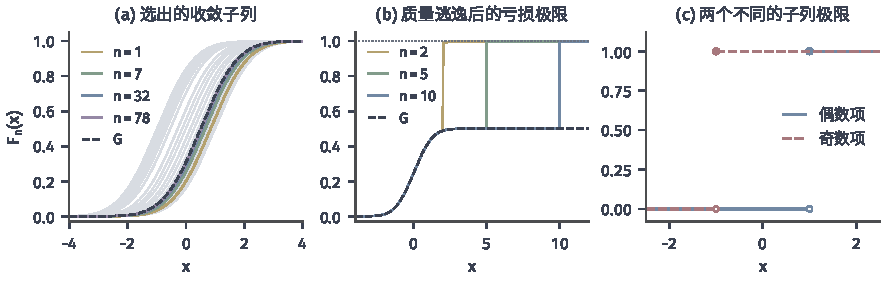
\includegraphics[width=150mm]{figures/02-abstract-mathematics/02-probability-spaces/matplotlib/wlim-helly-selection/figure.pdf}
  \caption{分布函数的子列选择。(a) $P_n=N(\sin n,1)$，灰线为$n=1,\ldots,30$的分布函数，彩色为均值依次接近$0.5$的项（$n=1,7,32,78$，均值约为$0.84,0.66,0.55,0.51$），虚线为极限$\Phi(x-0.5)$。(b) $P_n=\tfrac12N(0,1)+\tfrac12\delta_n$的分布函数（$n=2,5,10$）逐点趋于$G=\tfrac12\Phi$（虚线），$G(\infty)=1/2$。(c) $P_n=\delta_{(-1)^n}$，偶数项与奇数项的分布函数分别等于$\delta_1$与$\delta_{-1}$的分布函数。}
  \label{fig:wlim-helly-selection}
\end{figure*}

\paragraph{Prokhorov定理}
实轴上的构造推广到Polish空间，结论是子列存在与一致紧性等价。

\begin{theorem}[\term{Prokhorov定理}]
\label{thm:wlim-prokhorov}
设$S$是Polish空间，$\Pi$是$S$上的Borel概率测度族。则$\Pi$一致紧，当且仅当$\Pi$中每个序列都有弱收敛到某个Borel概率测度的子列。所得的极限不必属于$\Pi$。
\end{theorem}

一致紧推出子列存在的方向，实轴情形就是定理~\ref{thm:wlim-real-subsequence}；$\mathbb R^d$上可以用多元分布函数在有理点处作同样的对角线选择。
一般Polish空间的证明保留同一思路：先取一列紧集$K_m$使$\sup_{P\in\Pi}P(S\setminus K_m)<1/m$；在每个$K_m$中取可数稠密集，以其中的点为心、有理数为半径的闭球作有限并，得到一个可数集合族；对这个可数族作对角线选择，使子列在每个集合上的概率都收敛；再由这些极限值构造外测度，验证它限制在Borel集上是测度，并对每个开集满足Portmanteau定理中的下极限不等式。一致紧性保证构造出的测度总质量为一。完整论证可参考Kallenberg的概率论教材\scite{math-kallenberg2021probability}。

反方向的证明较短，我们完整写出。设$\Pi$中每个序列都有弱收敛子列，取$S$的可数稠密子集$\{s_j\}$，记开集$G_{m,N}=\bigcup_{j\leq N}B(s_j,1/m)$，固定$\varepsilon>0$。
我们断言：对每个$m$，存在$N_m$使$P(G_{m,N_m})>1-\varepsilon2^{-m}$对所有$P\in\Pi$成立。
否则存在$m$，对每个$N$都能取$P_N\in\Pi$使$P_N(G_{m,N})\leq1-\varepsilon2^{-m}$。按假设取子列$P_{N_k}\Rightarrow Q$。对固定的$N$，当$N_k\geq N$时$G_{m,N}\subseteq G_{m,N_k}$，由定理~\ref{thm:wlim-portmanteau}的开集判据，
\[
  Q(G_{m,N})\leq\liminf_kP_{N_k}(G_{m,N})\leq\liminf_kP_{N_k}(G_{m,N_k})\leq1-\varepsilon2^{-m}.
\]
但$G_{m,N}$随$N$增大到整个$S$，令$N\to\infty$得$Q(S)<1$，矛盾。
于是令$K=\bigcap_m\overline{G_{m,N_m}}$。与定理~\ref{thm:wlim-polish-tight}的证明一样，$K$闭且全有界，在完备空间中紧，并且$P(S\setminus K)\leq\sum_m\varepsilon2^{-m}=\varepsilon$对所有$P\in\Pi$成立。

\paragraph{从子列到整列}
Prokhorov定理只给出子列。要证明整列收敛，还需要下面的子列原理。

\begin{lemma}[子列原理]
\label{lem:wlim-subsequence-principle}
设$P_n,P$是度量空间上的Borel概率测度。若$\{P_n\}$的每个子列都有进一步的子列弱收敛到同一个$P$，则$P_n\Rightarrow P$。
\end{lemma}

\begin{proof}
若不然，存在$h\in C_b(S)$、$\varepsilon>0$与子列$n_k$，使$|\int h\,dP_{n_k}-\int h\,dP|\geq\varepsilon$对所有$k$成立。这个子列的任何进一步子列都不能弱收敛到$P$，与假设矛盾。
\end{proof}

由此得到证明整列弱收敛的标准路线：先证明一致紧，由Prokhorov定理知道每个子列都有弱收敛的进一步子列；再证明所有可能的子列极限都等于同一个$P$；最后由子列原理得到$P_n\Rightarrow P$。
第二步不能省略。图~\ref{fig:wlim-helly-selection}(c)中的$P_n=\delta_{(-1)^n}$全部集中在紧集$[-1,1]$上，一致紧；偶数项弱收敛到$\delta_1$，奇数项弱收敛到$\delta_{-1}$，两个子列极限不同，整列不收敛。
识别子列极限需要一种能够唯一确定分布、又便于取极限的工具，下一节的特征函数承担这个任务。

\section{概率分布的积分变换}
\label{sec:wlim-characteristic}

上一节留下的问题是识别子列极限。直接比较分布并不方便：独立随机变量之和的分布要用二重积分计算，逐个识别子列极限更无从下手。
本节把每个概率分布$P$变成一个确定的函数$\varphi_P$，这一函数把独立和变成乘积，唯一确定分布，并且其逐点收敛在适当条件下等价于弱收敛。
需要区分两种变换：这里的$P\mapsto\varphi_P$输出一个复值函数；下一节的推前$P\mapsto g_\#P$输出另一个概率分布。
所需工具只有复指数、第~\ref{chap:measure-spaces}章的积分与积分极限，以及上一节的紧性与弱子列，不预设一般Fourier分析或复分析。

\subsection{特征函数的定义与运算}

\paragraph{复值函数的积分}
对实数$\theta$，复指数$e^{i\theta}=\cos\theta+i\sin\theta$满足$|e^{i\theta}|=1$、$e^{i(\theta+\eta)}=e^{i\theta}e^{i\eta}$，其共轭是$e^{-i\theta}$。
对复值可测函数$f=u+iv$，若$|f|$可积（等价地，$u$与$v$都可积），定义$\int f\,d\mu=\int u\,d\mu+i\int v\,d\mu$。这一积分对复系数线性，控制收敛定理可以分别用于实部与虚部。
我们还需要不等式$|\int f\,d\mu|\leq\int|f|\,d\mu$：若$\int f\,d\mu=re^{i\alpha}$，$r\geq0$，则
\[
  r=e^{-i\alpha}\int f\,d\mu=\int\operatorname{Re}\bigl(e^{-i\alpha}f\bigr)\,d\mu\leq\int|f|\,d\mu,
\]
中间一步用到$r$是实数，所以虚部的积分为零。
最后，若$X\perp Y$，$f,g$是有界复值可测函数，把$f(X)g(Y)$的实部与虚部展开成四个实值乘积，分别应用定理~\ref{thm:pmod-product-expectation}，得到$\mathbb E[f(X)g(Y)]=\mathbb E f(X)\,\mathbb E g(Y)$。

\paragraph{特征函数的定义}
复指数$x\mapsto e^{itx}$有界连续，它对任何概率分布都可积。

\begin{definition}[特征函数]
\label{def:wlim-characteristic}
设$P$是$\mathbb R$上的Borel概率测度，称
\[
  \varphi_P(t)=\int_{\mathbb R}e^{itx}\,P(dx),\qquad t\in\mathbb R,
\]
为$P$的\term{特征函数}（characteristic function）。若实值随机变量$X$的分布为$P$，记$\varphi_X(t)=\mathbb E\,e^{itX}=\varphi_P(t)$。
对$\mathbb R^d$上的概率测度和$\mathbb R^d$值随机向量$\bm X$，相应地定义$\varphi_{\bm X}(\bm t)=\mathbb E\,e^{i\langle\bm t,\bm X\rangle}$，$\bm t\in\mathbb R^d$。
\end{definition}

特征函数只依赖分布，同分布的随机变量有相同的特征函数。下面的基本性质对任何分布成立，不要求均值或方差有限。

\begin{theorem}[特征函数的基本性质]
\label{thm:wlim-chf-basic}
设$\varphi$是$\mathbb R^d$上某个概率测度的特征函数，则$\varphi(\bm 0)=1$，$|\varphi(\bm t)|\leq1$，$\varphi(-\bm t)=\overline{\varphi(\bm t)}$，并且$\varphi$在$\mathbb R^d$上一致连续。
\end{theorem}

\begin{proof}
前三条分别来自$e^{0}=1$、$|\int f\,dP|\leq\int|f|\,dP$与$e^{-i\theta}=\overline{e^{i\theta}}$。对一致连续性，
\[
  |\varphi(\bm t+\bm s)-\varphi(\bm t)|=\Bigl|\mathbb E\bigl[e^{i\langle\bm t,\bm X\rangle}(e^{i\langle\bm s,\bm X\rangle}-1)\bigr]\Bigr|\leq\mathbb E\bigl|e^{i\langle\bm s,\bm X\rangle}-1\bigr|.
\]
右端与$\bm t$无关。当$\bm s\to\bm 0$时被积函数逐点趋于零且以$2$为界，由控制收敛定理趋于零。
\end{proof}

由第三条性质，若$X$与$-X$同分布，则$\varphi_X(t)=\varphi_{-X}(t)=\varphi_X(-t)=\overline{\varphi_X(t)}$，特征函数是实值的，这时它等于$\mathbb E\cos(tX)$。

\paragraph{仿射变换与独立和}
特征函数的用处首先在于运算规则简单。

\begin{theorem}[仿射变换与独立和]
\label{thm:wlim-chf-operations}
设$\bm X$是$\mathbb R^d$值随机向量。
\begin{enumerate}
  \item 对$m\times d$矩阵$\bm A$与$\bm b\in\mathbb R^m$，$\varphi_{\bm A\bm X+\bm b}(\bm t)=e^{i\langle\bm t,\bm b\rangle}\varphi_{\bm X}(\bm A^\top\bm t)$；特别地，实值情形$\varphi_{aX+b}(t)=e^{itb}\varphi_X(at)$。
  \item 若$\bm X\perp\bm Y$且二者都取值于$\mathbb R^d$，则$\varphi_{\bm X+\bm Y}=\varphi_{\bm X}\varphi_{\bm Y}$。
\end{enumerate}
\end{theorem}

\begin{proof}
第一条由$\langle\bm t,\bm A\bm X+\bm b\rangle=\langle\bm A^\top\bm t,\bm X\rangle+\langle\bm t,\bm b\rangle$及$e^{i(\theta+\eta)}=e^{i\theta}e^{i\eta}$得到。
第二条中$e^{i\langle\bm t,\bm X+\bm Y\rangle}=e^{i\langle\bm t,\bm X\rangle}e^{i\langle\bm t,\bm Y\rangle}$，两个因子分别是$\bm X$与$\bm Y$的有界复值函数，由独立性下的乘积公式即得。
\end{proof}

独立和的分布本身是一个二重积分。由定理~\ref{thm:pmod-independence-product}，$(\bm X,\bm Y)$的联合分布是乘积测度$P_{\bm X}\otimes P_{\bm Y}$，用Fubini定理得
\[
  \mathbb P(\bm X+\bm Y\in B)=\int P_{\bm Y}(B-\bm x)\,P_{\bm X}(d\bm x),\qquad B-\bm x=\{\bm y-\bm x:\bm y\in B\}.
\]
这个分布称为$P_{\bm X}$与$P_{\bm Y}$的\term{卷积}（convolution），记作$P_{\bm X}*P_{\bm Y}$。逐次计算$n$重卷积很繁琐，而定理~\ref{thm:wlim-chf-operations}说明它的特征函数只是各因子的乘积，中心极限定理的证明正是利用这一点。

乘积规则依赖独立性，不相关不够。设$X$在$\{-1,0,1\}$上均匀分布，$Y=\mathbb I_{\{X=0\}}$。由于$XY=0$恒成立且$\mathbb E X=0$，$\operatorname{Cov}(X,Y)=0$。
但$X+Y$以概率$1/3$取$-1$、以概率$2/3$取$1$，在$t=\pi$处$\varphi_{X+Y}(\pi)=-1$；而$\varphi_X(\pi)=(1+2\cos\pi)/3=-1/3$，$\varphi_Y(\pi)=2/3+e^{i\pi}/3=1/3$，乘积为$-1/9$。

\paragraph{几个常见分布的特征函数}
下面的计算将在后文反复使用。
若$X\sim\operatorname{Bernoulli}(p)$，则$\varphi_X(t)=1-p+pe^{it}$；二项分布$\operatorname{Bin}(n,p)$是$n$个独立Bernoulli变量之和，特征函数为$(1-p+pe^{it})^n$。
Rademacher变量$R$以相等概率取$\pm1$，$\varphi_R(t)=\cos t$。$\mathrm{Unif}[-1,1]$的特征函数是$\frac12\int_{-1}^1e^{itx}\,dx=\sin t/t$（$t\ne0$），在$t=0$处取$1$。

标准正态分布的特征函数需要稍作推导。记$\phi(x)=e^{-x^2/2}/\sqrt{2\pi}$。分布对称，故$\varphi(t)=\int\cos(tx)\phi(x)\,dx$。
由$|\cos a-\cos b|\leq|a-b|$，差商$[\cos((t+s)x)-\cos(tx)]/s$以$|x|$为界，而$|x|\phi(x)$可积，由控制收敛定理可以在积分号下求导；再用$\phi'(x)=-x\phi(x)$分部积分，
\[
  \varphi'(t)=-\int x\sin(tx)\phi(x)\,dx=\int\sin(tx)\phi'(x)\,dx=-t\varphi(t),
\]
边界项$\sin(tx)\phi(x)$在$\pm\infty$处为零。于是$(\varphi(t)e^{t^2/2})'=0$，结合$\varphi(0)=1$得
\begin{equation}
  \varphi_{N(0,1)}(t)=e^{-t^2/2}.
  \label{eq:wlim-normal-chf}
\end{equation}
由仿射规则，$N(\mu,\sigma^2)$的特征函数是$e^{i\mu t-\sigma^2t^2/2}$。两个独立正态变量$N(\mu_1,\sigma_1^2)$与$N(\mu_2,\sigma_2^2)$之和的特征函数是$e^{i(\mu_1+\mu_2)t-(\sigma_1^2+\sigma_2^2)t^2/2}$，正是$N(\mu_1+\mu_2,\sigma_1^2+\sigma_2^2)$的特征函数；待下一小节证明唯一性后，这就推出独立正态之和仍是正态。

多元正态分布也可以由此确定。设$\bm\Sigma$是$d\times d$半正定矩阵，取矩阵$\bm A$使$\bm A\bm A^\top=\bm\Sigma$，$\bm Z$的$d$个坐标独立且服从$N(0,1)$。称$\bm\mu+\bm A\bm Z$的分布为$N(\bm\mu,\bm\Sigma)$。由仿射规则和坐标独立，
\begin{equation}
  \varphi_{N(\bm\mu,\bm\Sigma)}(\bm t)=e^{i\langle\bm t,\bm\mu\rangle}\prod_{j=1}^de^{-(\bm A^\top\bm t)_j^2/2}=\exp\Bigl(i\langle\bm t,\bm\mu\rangle-\tfrac12\bm t^\top\bm\Sigma\bm t\Bigr).
  \label{eq:wlim-mvn-chf}
\end{equation}
右端只依赖$\bm\mu$与$\bm\Sigma$，唯一性定理证明后即知$N(\bm\mu,\bm\Sigma)$不依赖$\bm A$的选取。$\bm\Sigma$奇异时$\bm A$不满秩，分布集中在一个低维仿射子空间上，没有密度，但特征函数公式照样成立。

图~\ref{fig:wlim-characteristic-functions}(a)比较三个对称分布的特征函数：它们都是实值偶函数，在原点取$1$。Rademacher分布的$\cos t$周期性地回到$\pm1$，这对应于取值只在整数格点上的离散分布；均匀分布的$\sin t/t$在远处振荡衰减；正态分布的$e^{-t^2/2}$衰减最快。
(b)中Bernoulli$(0.3)$分布不对称，特征函数有非零虚部；它的模$|0.7+0.3e^{it}|$在$0.4$与$1$之间周期变化。

\begin{figure}[htbp]
  \centering
  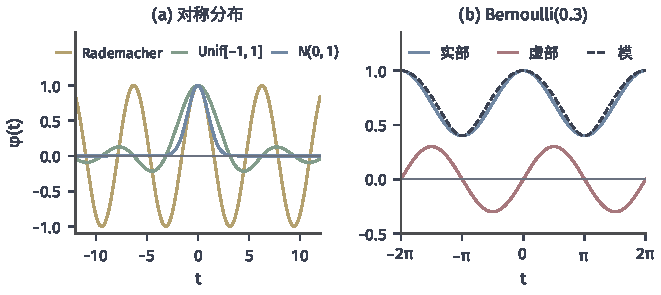
\includegraphics[width=112mm]{figures/02-abstract-mathematics/02-probability-spaces/matplotlib/wlim-characteristic-functions/figure.pdf}
  \caption{几个分布的特征函数。(a) Rademacher分布$\cos t$、$\mathrm{Unif}[-1,1]$分布$\sin t/t$与标准正态分布$e^{-t^2/2}$，三者都是实值偶函数。(b) $\operatorname{Bernoulli}(0.3)$分布的特征函数$0.7+0.3e^{it}$的实部、虚部与模，周期为$2\pi$，模的最小值为$0.4$。}
  \label{fig:wlim-characteristic-functions}
\end{figure}

\subsection{特征函数与矩}

\paragraph{矩条件下的求导}
特征函数在原点附近的行为记录了分布的矩。我们先说明有限绝对矩怎样给出可微性。证明反复使用不等式$|e^{iu}-1|=|\int_0^uie^{is}\,ds|\leq|u|$，$u\in\mathbb R$。

\begin{theorem}[有限矩与导数]
\label{thm:wlim-chf-derivatives}
设$X$是实值随机变量，$m$为正整数，$\mathbb E|X|^m<\infty$。则$\varphi_X$在$\mathbb R$上$m$阶连续可导，并且对$1\leq k\leq m$，
\[
  \varphi_X^{(k)}(t)=\mathbb E\bigl[(iX)^ke^{itX}\bigr],\qquad\text{特别地}\quad\mathbb E X^k=i^{-k}\varphi_X^{(k)}(0).
\]
\end{theorem}

\begin{proof}
由定理~\ref{thm:pmod-moment-monotone}，$\mathbb E|X|^k<\infty$对$k\leq m$成立。对$k$归纳，设$\varphi_X^{(k-1)}(t)=\mathbb E[(iX)^{k-1}e^{itX}]$（$k=1$时即定义）。对$s\neq0$，
\[
  \frac{\varphi_X^{(k-1)}(t+s)-\varphi_X^{(k-1)}(t)}{s}=\mathbb E\Bigl[(iX)^{k-1}e^{itX}\,\frac{e^{isX}-1}{s}\Bigr].
\]
期望内的量当$s\to0$时逐点趋于$(iX)^ke^{itX}$，模不超过$|X|^{k-1}\cdot|X|=|X|^k$，后者可积。沿任一趋于零的数列$s_j$用控制收敛定理，即得导数公式。
导数$\mathbb E[(iX)^ke^{itX}]$关于$t$连续，同样由控制收敛定理（控制函数$|X|^k$）得到。
\end{proof}

定理只建立了“有限绝对矩推出可微”这一方向。反过来由导数存在推出矩有限需要另外的论证，对奇数阶一般不成立，本章不使用。

\paragraph{二阶展开}
中心极限定理只需要特征函数在原点的二阶展开，而且只需要有限二阶矩。关键是复指数Taylor余项的一个双重估计。

\begin{lemma}[复指数的二阶余项]
\label{lem:wlim-exp-remainder}
对实数$u$，
\[
  \Bigl|e^{iu}-1-iu+\frac{u^2}2\Bigr|\leq\min\Bigl\{\frac{|u|^3}6,\,u^2\Bigr\}.
\]
\end{lemma}

\begin{proof}
设$u\geq0$（$u<0$时取共轭）。由$e^{is}-1=i\int_0^se^{ir}\,dr$并交换积分次序，
\[
  e^{iu}-1-iu=i\int_0^u(e^{is}-1)\,ds=-\int_0^u\!\!\int_0^se^{ir}\,dr\,ds=-\int_0^u(u-r)e^{ir}\,dr.
\]
又$\int_0^u(u-r)\,dr=u^2/2$，所以$e^{iu}-1-iu+u^2/2=-\int_0^u(u-r)(e^{ir}-1)\,dr$。
用$|e^{ir}-1|\leq r$得到上界$\int_0^u(u-r)r\,dr=u^3/6$；用$|e^{ir}-1|\leq2$得到上界$u^2$。
\end{proof}

\begin{theorem}[有限二阶矩下的展开]
\label{thm:wlim-chf-second-order}
设$\mathbb E X^2<\infty$，则当$t\to0$时
\[
  \varphi_X(t)=1+it\,\mathbb E X-\frac{t^2}2\,\mathbb E X^2+o(t^2).
\]
特别地，若$\mathbb E X=0$、$\operatorname{Var}X=\sigma^2$，则$\varphi_X(t)=1-\sigma^2t^2/2+o(t^2)$。
设$\bm X$是均值为$\bm\mu$、协方差矩阵为$\bm\Sigma$的$\mathbb R^d$值随机向量，则对固定方向$\bm a\in\mathbb R^d$，当$u\to0$时
\[
  \varphi_{\bm X-\bm\mu}(u\bm a)=1-\frac{u^2}2\,\bm a^\top\bm\Sigma\bm a+o(u^2).
\]
\end{theorem}

\begin{proof}
记$R(u)=e^{iu}-1-iu+u^2/2$，则$\varphi_X(t)-(1+it\,\mathbb E X-\tfrac12t^2\,\mathbb E X^2)=\mathbb E\,R(tX)$。由引理~\ref{lem:wlim-exp-remainder}，
\[
  \frac{|R(tX)|}{t^2}\leq\min\Bigl\{\frac{|t|\,|X|^3}6,\,X^2\Bigr\}.
\]
右端当$t\to0$时逐点趋于零，并以可积的$X^2$为界，由控制收敛定理$\mathbb E|R(tX)|/t^2\to0$。
向量情形把一维结论用于$Y=\bm a^\top(\bm X-\bm\mu)$：$\mathbb E Y=0$，$\operatorname{Var}Y=\bm a^\top\bm\Sigma\bm a$，并且$\varphi_{\bm X-\bm\mu}(u\bm a)=\varphi_Y(u)$。
\end{proof}

证明中的二阶控制$X^2$来自余项估计的第二部分，三阶估计只用于说明逐点趋于零，因此不需要三阶矩。结论也不要求矩母函数存在。

\subsection{反演与分布唯一性}

\paragraph{截断反演积分}
特征函数能否唯一确定分布？在实轴上，我们直接由特征函数恢复区间概率。先准备一个正弦积分的极限。

\begin{lemma}[正弦积分]
\label{lem:wlim-sine-integral}
令$S(y)=\int_0^y\frac{\sin u}u\,du$，$y\in\mathbb R$。则$S$是连续的奇函数，在$\mathbb R$上有界，并且$S(y)\to\pi/2$（$y\to\infty$）。
\end{lemma}

\begin{proof}
被积函数在$u=0$处按连续延拓取$1$，所以$S$连续；被积函数是偶函数，故$S$是奇函数。
对$y>0$，用$1/u=\int_0^\infty e^{-us}\,ds$（$u>0$）写成二重积分。由于$\int_0^y\int_0^\infty|\sin u|e^{-us}\,ds\,du=\int_0^y|\sin u|/u\,du\leq y$，Fubini定理允许交换次序：
\[
  S(y)=\int_0^\infty\!\!\int_0^y\sin u\,e^{-us}\,du\,ds=\int_0^\infty\frac{1-e^{-ys}(s\sin y+\cos y)}{1+s^2}\,ds,
\]
内层积分对$y$求导即可验证。右端第一部分积分为$\pi/2$；第二部分的模不超过$\int_0^\infty e^{-ys}\frac{s+1}{1+s^2}\,ds\leq\frac2y$，因为$(s+1)/(1+s^2)\leq2$。所以$|S(y)-\pi/2|\leq2/y\to0$。
$S$在每个有界区间上连续因而有界，在$[2,\infty)$上又被$\pi/2+1$控制；由奇性，$S$在整条实轴上有界。
\end{proof}

\begin{theorem}[反演公式]
\label{thm:wlim-inversion}
设$P$是$\mathbb R$上的概率测度，$a<b$。则
\[
  \lim_{T\to\infty}\frac1{2\pi}\int_{-T}^T\frac{e^{-ita}-e^{-itb}}{it}\,\varphi_P(t)\,dt=P\bigl((a,b)\bigr)+\frac12P(\{a\})+\frac12P(\{b\}),
\]
其中被积函数在$t=0$处按连续延拓取值$b-a$。特别地，若$a,b$都不是$P$的原子，极限就是$P((a,b))$。
\end{theorem}

\begin{proof}
记左端截断积分为$I_T$。由$\bigl|\frac{e^{-ita}-e^{-itb}}{it}\bigr|=\bigl|\int_a^be^{-itu}\,du\bigr|\leq b-a$，被积函数在$[-T,T]\times\mathbb R$上有界，对有限测度$dt\otimes P$用Fubini定理交换积分：
\[
  I_T=\int_{\mathbb R}J_T(x)\,P(dx),\qquad J_T(x)=\frac1{2\pi}\int_{-T}^T\frac{e^{it(x-a)}-e^{it(x-b)}}{it}\,dt.
\]
把$e^{itc}/(it)$拆成$\cos(tc)/(it)+\sin(tc)/t$。余弦部分的差$[\cos(t(x-a))-\cos(t(x-b))]/(it)$是$t$的奇函数，在对称区间上积分为零；正弦部分是偶函数。代换$u=tc$得$\int_0^T\sin(tc)/t\,dt=S(Tc)$，于是
\[
  J_T(x)=\frac1\pi\Bigl[S\bigl(T(x-a)\bigr)-S\bigl(T(x-b)\bigr)\Bigr].
\]
由引理~\ref{lem:wlim-sine-integral}，当$T\to\infty$时$S(Tc)\to\frac\pi2\operatorname{sgn}c$，所以$J_T(x)$在$x<a$或$x>b$时趋于$0$，在$a<x<b$时趋于$1$，在$x=a$或$x=b$时趋于$1/2$。
$J_T$以$2\sup|S|/\pi$为界，对有限测度$P$用控制收敛定理，即得结论。
\end{proof}

图~\ref{fig:wlim-inversion-atom}(a)画出区间$(0,1)$对应的截断核$J_T$：$T$增大时它逼近区间的示性函数，但在两个端点处稳定地取$1/2$。
(b)以$\operatorname{Bernoulli}(0.3)$为例，原子在$0$（质量$0.7$）与$1$（质量$0.3$）。区间$(-0.5,0.5)$的端点不是原子，$I_T\to0.7=P((-0.5,0.5))$；区间$(0,1)$的两个端点都是原子，$I_T\to\frac12\cdot0.7+\frac12\cdot0.3=0.5$，既不是$P((0,1))=0$也不是$P([0,1])=1$；区间$(0,2)$只有左端点是原子，极限为$0.35+0.3=0.65$。
所以反演公式不要求分布有密度，但含原子的端点只能恢复半个质量。

\begin{figure}[htbp]
  \centering
  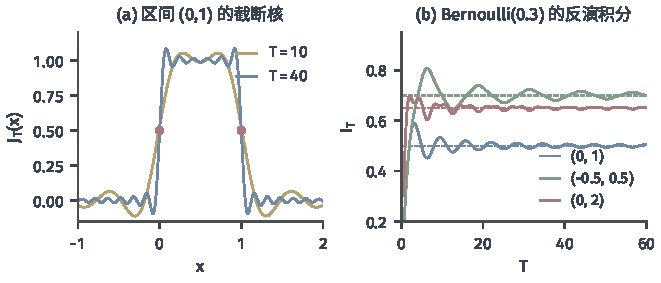
\includegraphics[width=112mm]{figures/02-abstract-mathematics/02-probability-spaces/matplotlib/wlim-inversion-atom/figure.pdf}
  \caption{截断反演积分在原子端点处给出半个质量。(a) 区间$(a,b)=(0,1)$的截断核$J_T(x)=[S(T(x-a))-S(T(x-b))]/\pi$，$T=10,40$，红点标出端点处的值$1/2$。(b) $P=\operatorname{Bernoulli}(0.3)$时三个区间的截断积分$I_T$随$T$的变化，虚线为反演公式给出的极限$0.5$、$0.7$与$0.65$。}
  \label{fig:wlim-inversion-atom}
\end{figure}

\paragraph{实轴上的唯一性}
反演公式立即说明，实轴上特征函数相同的两个分布相同。
设$\varphi_P=\varphi_Q$。两者原子合起来至多可数，对不是任一原子的$a<b$，反演公式给出$P((a,b))=Q((a,b))$。
令$a$沿非原子点趋于$-\infty$，得$P((-\infty,b))=Q((-\infty,b))$，对所有非原子点$b$成立；非原子点在实轴上稠密，从右侧逼近任一点$x$，由下连续性得$F_P(x)=F_Q(x)$，再由引理~\ref{lem:wlim-quantile-construction}中的唯一性部分得$P=Q$。

\paragraph{有限维的高斯平滑}
在$\mathbb R^d$上也可以写出多维区间的反演公式，但边界上的原子处理起来很繁琐。我们改用另一条路：给分布加上一点独立的高斯噪声，使它有一个由特征函数显式表示的密度，再让噪声消失。

\begin{lemma}[高斯平滑后的密度]
\label{lem:wlim-gaussian-smoothing}
设$\bm X$的分布为$P$，$\bm Z\sim N(\bm 0,\bm I_d)$与$\bm X$独立，$\varepsilon>0$。则$\bm X+\varepsilon\bm Z$有密度
\[
  g_\varepsilon(\bm y)=\frac1{(2\pi)^d}\int_{\mathbb R^d}e^{-i\langle\bm t,\bm y\rangle}e^{-\varepsilon^2\lVert\bm t\rVert^2/2}\varphi_P(\bm t)\,d\bm t.
\]
\end{lemma}

\begin{proof}
记$\phi_d$为$N(\bm 0,\bm I_d)$的密度。对Borel集$B$，由独立性、换元$\bm y=\bm x+\varepsilon\bm z$与Tonelli定理，
\[
  \begin{aligned}
  \mathbb P(\bm X+\varepsilon\bm Z\in B)&=\int\!\!\int\mathbb I_B(\bm x+\varepsilon\bm z)\phi_d(\bm z)\,d\bm z\,P(d\bm x)\\
  &=\int_B\int\varepsilon^{-d}\phi_d\Bigl(\frac{\bm y-\bm x}\varepsilon\Bigr)P(d\bm x)\,d\bm y.
  \end{aligned}
\]
把式~\eqref{eq:wlim-normal-chf}写成$\int e^{isw}\phi(w)\,dw=e^{-s^2/2}=\sqrt{2\pi}\,\phi(s)$，代换$w=\varepsilon\tau$、$s=v/\varepsilon$得$\varepsilon^{-1}\phi(v/\varepsilon)=\frac1{2\pi}\int e^{iv\tau}e^{-\varepsilon^2\tau^2/2}\,d\tau$；对$d$个坐标相乘，
\[
  \varepsilon^{-d}\phi_d\Bigl(\frac{\bm v}\varepsilon\Bigr)=\frac1{(2\pi)^d}\int e^{-i\langle\bm t,\bm v\rangle}e^{-\varepsilon^2\lVert\bm t\rVert^2/2}\,d\bm t,
\]
其中把$\bm t$换成$-\bm t$不改变积分。代入$\bm v=\bm y-\bm x$，被积函数的模不超过可积的$e^{-\varepsilon^2\lVert\bm t\rVert^2/2}$，用Fubini定理先对$P(d\bm x)$积分，$\int e^{i\langle\bm t,\bm x\rangle}P(d\bm x)=\varphi_P(\bm t)$，即得所述密度。
\end{proof}

\begin{theorem}[特征函数的唯一性]
\label{thm:wlim-uniqueness}
设$P,Q$是$\mathbb R^d$上的Borel概率测度。若$\varphi_P(\bm t)=\varphi_Q(\bm t)$对所有$\bm t\in\mathbb R^d$成立，则$P=Q$。
\end{theorem}

\begin{proof}
取$\bm X\sim P$、$\bm Y\sim Q$，各自配上独立的$\bm Z\sim N(\bm 0,\bm I_d)$。由引理~\ref{lem:wlim-gaussian-smoothing}，$\bm X+\varepsilon\bm Z$与$\bm Y+\varepsilon\bm Z$的密度由同一公式给出，二者同分布。
对$h\in C_b(\mathbb R^d)$，于是$\mathbb E\,h(\bm X+\varepsilon\bm Z)=\mathbb E\,h(\bm Y+\varepsilon\bm Z)$。令$\varepsilon\downarrow0$，被积量逐点收敛且有界，由控制收敛定理得$\int h\,dP=\int h\,dQ$；再由引理~\ref{lem:wlim-uniqueness-limit}，$P=Q$。
\end{proof}

这条证明对$d=1$同样适用，它没有用到下一节的Cramér--Wold判据，也没有预设一般的Fourier反演定理。高斯平滑把“特征函数相同”变成“平滑后的密度相同”，有界连续测试再把平滑撤去。

\subsection{特征函数与弱收敛}

\paragraph{弱收敛推出逐点收敛}
若$P_n\Rightarrow P$，对固定的$\bm t$，$\cos\langle\bm t,\bm x\rangle$与$\sin\langle\bm t,\bm x\rangle$都是有界连续函数，所以$\varphi_{P_n}(\bm t)\to\varphi_P(\bm t)$。
我们真正需要的是反方向：只知道特征函数逐点收敛，能否断定分布弱收敛，甚至在事先没有候选极限的情况下找到极限？

\paragraph{L\'evy连续性定理}
答案是肯定的，只需在原点处加一个连续性条件。

\begin{theorem}[\term{L\'evy连续性定理}]
\label{thm:wlim-levy}
设$P_n$是$\mathbb R^d$上的概率测度。
\begin{enumerate}
  \item 若$P_n\Rightarrow P$，则$\varphi_{P_n}(\bm t)\to\varphi_P(\bm t)$对每个$\bm t$成立。
  \item 若对每个$\bm t$，$\varphi_{P_n}(\bm t)$收敛到某个数$\varphi(\bm t)$，并且函数$\varphi$在$\bm 0$处连续，则存在概率测度$P$使$\varphi=\varphi_P$，并且$P_n\Rightarrow P$。
\end{enumerate}
\end{theorem}

第二条不要求预先给出候选极限，极限$P$由定理本身产生。原点连续性不能删去。

\begin{example}[方差趋于无穷的正态分布]
\label{ex:wlim-spreading-normal}
令$P_n=N(0,n)$，则$\varphi_{P_n}(t)=e^{-nt^2/2}$，其逐点极限$\varphi(t)$在$t=0$处为$1$、其余点为$0$，在原点不连续。
相应地，分布函数$F_n(x)=\Phi(x/\sqrt n)\to1/2$对每个$x$成立，极限不是任何分布函数：质量同时向两侧无穷远逃逸，$\{P_n\}$不一致紧，也没有弱收敛到概率测度的子列。
\end{example}

图~\ref{fig:wlim-levy-counterexample}对照了两面：(a)中特征函数越来越窄，只在原点保留高度$1$；(b)中分布函数越来越平，压向高度$1/2$的水平线。
特征函数在原点附近的急剧下降，正是分布在远处有大量质量的信号；下面的引理把这一对应写成不等式。

\begin{figure}[htbp]
  \centering
  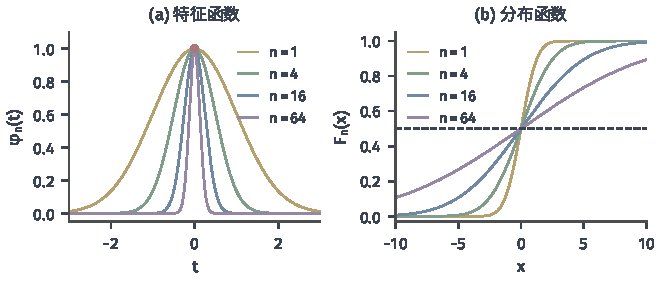
\includegraphics[width=112mm]{figures/02-abstract-mathematics/02-probability-spaces/matplotlib/wlim-levy-counterexample/figure.pdf}
  \caption{$P_n=N(0,n)$的特征函数与分布函数，$n=1,4,16,64$。(a) $\varphi_n(t)=e^{-nt^2/2}$的逐点极限在原点为$1$（红点）、其余点为$0$。(b) $F_n(x)=\Phi(x/\sqrt n)$逐点趋于$1/2$（虚线），不存在概率分布极限。}
  \label{fig:wlim-levy-counterexample}
\end{figure}

\paragraph{原点附近的积分控制}
\begin{lemma}[尾部概率的特征函数界]
\label{lem:wlim-tail-bound}
设$P$是$\mathbb R$上的概率测度，$u>0$。则
\[
  P\Bigl(\bigl\{x:|x|>\tfrac2u\bigr\}\Bigr)\leq\frac1u\int_{-u}^u\bigl(1-\varphi_P(t)\bigr)\,dt.
\]
\end{lemma}

\begin{proof}
对$x\neq0$，$\frac1u\int_{-u}^u(1-e^{itx})\,dt=2-\frac{2\sin(ux)}{ux}$，对$x=0$该积分为$0$。被积函数有界，用Fubini定理交换积分次序，
\[
  \frac1u\int_{-u}^u\bigl(1-\varphi_P(t)\bigr)\,dt=\int_{\mathbb R}\Bigl(2-\frac{2\sin(ux)}{ux}\Bigr)P(dx).
\]
由$|\sin y|\leq|y|$，右端被积函数非负；当$|ux|\geq2$时$|\sin(ux)/(ux)|\leq1/2$，被积函数至少为$1$。所以右端不小于$P(|x|\geq2/u)$。
\end{proof}

左端只用到$\varphi_P$在区间$[-u,u]$上的值：$u$越小，看到的是越远处的尾部。

\paragraph{连续性定理的证明}
定理~\ref{thm:wlim-levy}的第一条前面已经证明。第二条按“原点附近的积分控制、一致紧性、弱收敛子列、极限唯一”四步完成。

\begin{proof}[定理~\ref{thm:wlim-levy}第二条的证明]
先设$d=1$。由$\varphi_{P_n}(0)=1$得$\varphi(0)=1$。固定$\varepsilon>0$，由$\varphi$在原点连续，取$u>0$使$|1-\varphi(t)|<\varepsilon/2$对$|t|\leq u$成立，于是$\frac1u\int_{-u}^u|1-\varphi(t)|\,dt\leq\varepsilon$。
在$[-u,u]$上$|1-\varphi_{P_n}|\leq2$且逐点趋于$1-\varphi$，由控制收敛定理，
\[
  \frac1u\int_{-u}^u\bigl(1-\varphi_{P_n}(t)\bigr)\,dt\to\frac1u\int_{-u}^u\bigl(1-\varphi(t)\bigr)\,dt,
\]
后者的模不超过$\varepsilon$。所以存在$N$，当$n\geq N$时左端小于$2\varepsilon$，由引理~\ref{lem:wlim-tail-bound}得$P_n(|x|>2/u)<2\varepsilon$。前$N-1$个测度各自是紧的，把半径增大即可覆盖，于是$\{P_n\}$一致紧。

对一般$d$，第$j$个坐标在$P_n$下的特征函数是$s\mapsto\varphi_{P_n}(s\bm e_j)$，它逐点收敛到在$s=0$处连续的$\varphi(s\bm e_j)$。由一维情形，每个坐标的分布族一致紧；再由
\[
  P_n\bigl(\lVert\bm x\rVert_\infty>R\bigr)\leq\sum_{j=1}^dP_n(|x_j|>R),
\]
联合分布族一致紧。

由Prokhorov定理（定理~\ref{thm:wlim-prokhorov}），每个子列都有进一步的子列$P_{n_k}\Rightarrow Q$，$Q$是某个概率测度。由第一条，$\varphi_{P_{n_k}}\to\varphi_Q$逐点成立；而$\varphi_{P_{n_k}}\to\varphi$，所以$\varphi_Q=\varphi$。
任何两个子列极限都有特征函数$\varphi$，由定理~\ref{thm:wlim-uniqueness}它们是同一个测度$P$，且$\varphi=\varphi_P$。最后由子列原理（引理~\ref{lem:wlim-subsequence-principle}）得$P_n\Rightarrow P$。
\end{proof}

证明中坐标方向只负责一致紧性：坐标的尾部概率之和控制联合分布的尾部。识别联合极限时用的仍是全部$\bm t\in\mathbb R^d$上的特征函数，不能只由各坐标的边缘收敛代替。

\subsection{矩母函数及其适用条件（补充）}

\paragraph{有限域与各阶矩}
初等概率中常用矩母函数计算矩、识别分布。它和特征函数的区别在于指数是实的，因而可能发散。
对实值随机变量$X$，令$M_X(t)=\mathbb E\,e^{tX}\in(0,\infty]$，称为\term{矩母函数}（moment generating function），其有限域为$D_X=\{t:M_X(t)<\infty\}$。
$0\in D_X$总成立，但这远不足以读取矩；需要的条件是$M_X$在零点的某个开邻域$(-t_0,t_0)$内有限。

在此条件下取$0<a<t_0$，由$e^{a|X|}\leq e^{aX}+e^{-aX}$得$\mathbb E\,e^{a|X|}<\infty$，各阶矩都有限。
对$|t|\leq a'<a$，$|X|^ke^{tX}\leq|X|^ke^{a'|X|}\leq C_ke^{a|X|}$，其中$C_k=\sup_{y\geq0}y^ke^{-(a-a')y}<\infty$。这个可积控制允许像定理~\ref{thm:wlim-chf-derivatives}那样逐阶把求导移入期望，得到$M_X^{(k)}(t)=\mathbb E[X^ke^{tX}]$，特别是$M_X^{(k)}(0)=\mathbb E X^k$。

\paragraph{矩母函数与分布唯一性}
若$M_X=M_Y$在$(-t_0,t_0)$内有限，则$X$与$Y$同分布。下面的论证只用实参数幂级数与积分交换。

先说明特征函数在每一点都有半径统一的Taylor展开。对实数$s$与$|h|<t_0$，由$|e^{iv}-\sum_{k<n}(iv)^k/k!|\leq|v|^n/n!$（与引理~\ref{lem:wlim-exp-remainder}同样由积分余项得到），
\[
  \Bigl|\varphi_X(s+h)-\sum_{k<n}\frac{(ih)^k}{k!}\mathbb E\bigl[X^ke^{isX}\bigr]\Bigr|\leq\frac{|h|^n\,\mathbb E|X|^n}{n!}.
\]
由$\sum_n|h|^n\mathbb E|X|^n/n!=\mathbb E\,e^{|h||X|}<\infty$，右端趋于零，由定理~\ref{thm:wlim-chf-derivatives}，$i^k\mathbb E[X^ke^{isX}]=\varphi_X^{(k)}(s)$，所以$\varphi_X(s+h)=\sum_kh^k\varphi_X^{(k)}(s)/k!$对$|h|<t_0$成立，半径$t_0$与$s$无关，因为$|e^{isX}|=1$。

在$s=0$处，展开系数是各阶矩，由前一段它们由$M_X$在零点的导数确定，所以$\varphi_X=\varphi_Y$在$(-t_0,t_0)$上成立。
若两个特征函数在某点$s$的邻域内相等，则它们在$s$处的各阶导数相等，展开式在$(s-t_0,s+t_0)$上相同。从$s=\pm t_0/2$出发，相等区间扩大到$(-3t_0/2,3t_0/2)$；如此每次延伸$t_0/2$，覆盖整条实轴。最后由定理~\ref{thm:wlim-uniqueness}得$X$与$Y$同分布。

\paragraph{各阶矩有限不能代替矩母函数有限}
条件“在零点邻域内有限”不能换成“各阶矩都有限”。
令$Z\sim N(0,1)$、$X=e^Z$。由配方，$e^{kz}\phi(z)=e^{k^2/2}\phi(z-k)$，所以$\mathbb E\,e^{kZ}=e^{k^2/2}$，$X$的各阶矩$\mathbb E X^k=e^{k^2/2}$都有限；但对$t>0$，$te^z-z^2/2\to\infty$（$z\to\infty$），所以$M_X(t)=\infty$，$D_X=(-\infty,0]$。
这时上面基于指数可积的唯一性论证无法启动。事实上，密度$f(x)\bigl(1+\sin(2\pi\log x)\bigr)$（$f$为$X$的密度）与$X$有完全相同的各阶矩：$\int x^kf(x)\sin(2\pi\log x)\,dx=\mathbb E[e^{kZ}\sin(2\pi Z)]=e^{k^2/2}\,\mathbb E\sin(2\pi(Z+k))=0$，其中第二步再次使用上述配方，最后一步用到$k$是整数及$Z$的对称性。各阶矩一般不能唯一确定分布，本章不展开这一问题。
后面的中心极限定理只用定理~\ref{thm:wlim-chf-second-order}的二阶展开，不需要矩母函数。

\section{联合分布与函数变换的极限}
\label{sec:wlim-joint-transform}

统计量很少是单个渐近量本身。学生化均值是一个分子除以一个分母，回归系数的估计是几个样本矩的组合。
本节研究几个随机量组成的联合分布怎样收敛，以及对它们作函数变换后极限怎样传递：先补足边缘分布不包含的配对信息，再建立连续变换、随机标准化和近似替换的规则。
这些规则都不以中心极限定理为前提，下一节证明中心极限定理后可以直接使用。

\subsection{联合分布的收敛判据}

\paragraph{边缘相同、配对不同}
设对每个$n$，$X_n$与$Y_n$定义在同一个概率空间上，组成随机向量$(X_n,Y_n)$。
联合分布记录两组取值怎样配对，边缘分布只分别记录各自的规律。第~\ref{chap:probability-models}章的例~\ref{ex:pmod-bernoulli-couplings}已经说明相同的边缘可以有不同的配对；这里关心的是这种差别对极限的影响。

\begin{example}[交替配对]
\label{ex:wlim-alternating-pairing}
设$Z$以相等概率取$\pm1$。$(Z,Z)$与$(Z,-Z)$的两个边缘都是$\pm1$上的均匀分布，但前者的坐标和是$2Z$，后者的坐标和恒为$0$。
令$n$为偶数时$(X_n,Y_n)=(Z,Z)$，$n$为奇数时$(X_n,Y_n)=(Z,-Z)$。两个边缘分布对所有$n$都不变，当然收敛；联合分布却在两种配对之间交替，不收敛，坐标和$X_n+Y_n$的分布也在两点分布与$\delta_0$之间交替。
\end{example}

图~\ref{fig:wlim-joint-pairings}用概率表并列两种配对：边缘行与边缘列完全相同，质量却分别落在对角线和反对角线上。
因此，不能由各个边缘的极限推断联合极限，更不能推断坐标之和、之积的极限；要对多个随机量作运算，先要得到联合分布的收敛。

\begin{figure}[htbp]
  \centering
  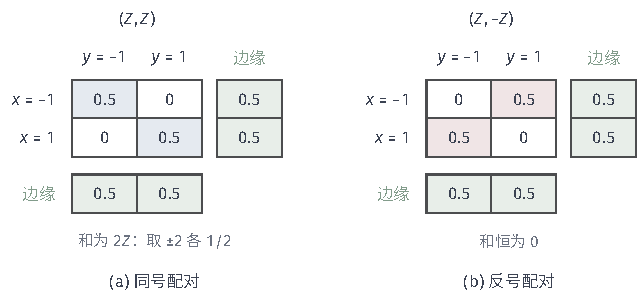
\includegraphics[width=108mm]{figures/02-abstract-mathematics/02-probability-spaces/tikz/wlim-joint-pairings/figure.pdf}
  \caption{边缘相同而联合分布不同的两种配对，$Z$以相等概率取$\pm1$。(a) $(Z,Z)$的联合概率表，质量在对角线上，坐标和为$2Z$。(b) $(Z,-Z)$的联合概率表，质量在反对角线上，坐标和恒为$0$。绿色单元是行边缘与列边缘，两种配对完全相同。}
  \label{fig:wlim-joint-pairings}
\end{figure}

\paragraph{Cram\'er--Wold判据}
联合分布的收敛可以化成一维问题，但要检验的不只是坐标，而是所有方向上的线性组合。

\begin{theorem}[\term{Cram\'er--Wold判据}]
\label{thm:wlim-cramer-wold}
设$\bm W_n,\bm W$是$\mathbb R^d$值随机向量。则$\bm W_n\Rightarrow\bm W$，当且仅当对每个$\bm a\in\mathbb R^d$都有$\bm a^\top\bm W_n\Rightarrow\bm a^\top\bm W$。
\end{theorem}

\begin{proof}
若$\bm W_n\Rightarrow\bm W$，对一维有界连续函数$h$，$\bm x\mapsto h(\bm a^\top\bm x)$在$\mathbb R^d$上有界连续，所以$\mathbb E\,h(\bm a^\top\bm W_n)\to\mathbb E\,h(\bm a^\top\bm W)$。
反过来，对每个$\bm a$，由一维弱收敛推出特征函数在$s=1$处收敛（定理~\ref{thm:wlim-levy}第一条）：
\[
  \varphi_{\bm W_n}(\bm a)=\mathbb E\,e^{i\bm a^\top\bm W_n}=\varphi_{\bm a^\top\bm W_n}(1)\to\varphi_{\bm a^\top\bm W}(1)=\varphi_{\bm W}(\bm a).
\]
所以向量特征函数逐点收敛到$\varphi_{\bm W}$，后者在原点连续。由定理~\ref{thm:wlim-levy}第二条，$\bm W_n$弱收敛到特征函数为$\varphi_{\bm W}$的分布，由唯一性这正是$\bm W$的分布。
\end{proof}

“所有方向”包括坐标的各种线性组合，只检验坐标方向不够。例~\ref{ex:wlim-alternating-pairing}中两个坐标方向的投影$X_n$与$Y_n$的分布都不变，但方向$\bm a=(1,1)$的投影$X_n+Y_n$不收敛。

\paragraph{行内独立时的乘积极限}
有一种常见情形无须逐个方向检验：同一行内的两组变量相互独立。

\begin{theorem}[行内独立的联合极限]
\label{thm:wlim-independent-product}
设对每个$n$，$\mathbb R^p$值的$\bm X_n$与$\mathbb R^q$值的$\bm Y_n$定义在同一概率空间上且相互独立。若$\bm X_n\Rightarrow P$、$\bm Y_n\Rightarrow Q$，则$(\bm X_n,\bm Y_n)\Rightarrow P\otimes Q$。
\end{theorem}

\begin{proof}
对$\bm s\in\mathbb R^p$、$\bm t\in\mathbb R^q$，由行内独立，
\[
  \varphi_{(\bm X_n,\bm Y_n)}(\bm s,\bm t)=\mathbb E\,e^{i\langle\bm s,\bm X_n\rangle}\,\mathbb E\,e^{i\langle\bm t,\bm Y_n\rangle}\to\varphi_P(\bm s)\varphi_Q(\bm t).
\]
由Fubini定理，右端正是乘积测度$P\otimes Q$的特征函数，它在原点连续，由定理~\ref{thm:wlim-levy}即得。
\end{proof}

定理要求的是每一行内部的独立性，不要求不同的$n$之间独立。若想用极限随机向量表述，应在乘积空间上取具有边缘$P$与$Q$的一对独立向量；随意取两个分别服从$P$与$Q$的变量，不能自动视为独立。

\subsection{连续函数变换下的分布极限}

\paragraph{连续映射保持弱收敛}
有了联合分布的极限，下一步是把它代入函数。设$S,T$是度量空间，$g:S\to T$可测，$P$在$g$下的推前$g_\#P$就是$g(X)$的分布，其中$X\sim P$。

\begin{theorem}[\term{连续映射定理}]
\label{thm:wlim-continuous-mapping}
设$S,T$是度量空间，$g:S\to T$连续。若$P_n\Rightarrow P$，则$g_\#P_n\Rightarrow g_\#P$；用随机对象表述，$X_n\Rightarrow X$推出$g(X_n)\Rightarrow g(X)$。
\end{theorem}

\begin{proof}
对$h\in C_b(T)$，$h\circ g\in C_b(S)$。由推前积分公式（式~\eqref{eq:measure-pushforward-integral}），
\[
  \int h\,d(g_\#P_n)=\int h\circ g\,dP_n\to\int h\circ g\,dP=\int h\,d(g_\#P),
\]
中间的极限来自$P_n\Rightarrow P$。
\end{proof}

证明中有界性由外层的$h$提供，所以$g$本身不必有界，例如$g(\bm x)=\lVert\bm x\rVert^2$。
坐标投影、范数和固定矩阵$\bm B$给出的线性变换$\bm x\mapsto\bm B\bm x$都是连续映射。对多个随机量，处理顺序总是先得到联合分布的极限，再代入连续函数：例如由$(X_n,Y_n)\Rightarrow(X,Y)$推出$X_n+Y_n\Rightarrow X+Y$、$X_nY_n\Rightarrow XY$；只有两个边缘的极限时，这一步无从谈起。

\paragraph{不连续点为零测集的映射}
阈值函数、比值等常用映射并非处处连续。只要不连续点在极限分布下概率为零，结论仍然成立。
记$D_g$为$g$的不连续点全体。它是Borel集：令$A_{m,k}$为满足“存在$y,z\in B(x,1/k)$使$d(g(y),g(z))\geq1/m$”的点$x$的集合，它是开集，而$D_g=\bigcup_m\bigcap_kA_{m,k}$。

\begin{theorem}[不连续点为零测集的连续映射]
\label{thm:wlim-continuous-mapping-ae}
设$g:S\to T$是Borel可测映射，$P_n\Rightarrow P$且$P(D_g)=0$，则$g_\#P_n\Rightarrow g_\#P$。
\end{theorem}

\begin{proof}
设$F\subseteq T$是闭集。若$x$属于$g^{-1}(F)$的闭包且$x\notin D_g$，取$x_k\in g^{-1}(F)$使$x_k\to x$，则$g(x_k)\to g(x)$，$F$闭推出$g(x)\in F$。所以$\overline{g^{-1}(F)}\subseteq g^{-1}(F)\cup D_g$。由定理~\ref{thm:wlim-portmanteau}，
\[
  \begin{aligned}
  \limsup_nP_n\bigl(g^{-1}(F)\bigr)&\leq\limsup_nP_n\bigl(\overline{g^{-1}(F)}\bigr)\leq P\bigl(\overline{g^{-1}(F)}\bigr)\\
  &\leq P\bigl(g^{-1}(F)\bigr)+P(D_g)=P\bigl(g^{-1}(F)\bigr).
  \end{aligned}
\]
即$\limsup_ng_\#P_n(F)\leq g_\#P(F)$，再用一次定理~\ref{thm:wlim-portmanteau}。
\end{proof}

以阈值函数$g(x)=\mathbb I_{\{x>c\}}$为例，$D_g=\{c\}$。若极限分布在$c$处没有原子，则$\mathbb I_{\{X_n>c\}}\Rightarrow\mathbb I_{\{X>c\}}$，即$\mathbb P(X_n>c)\to\mathbb P(X>c)$。
移动点质量$\delta_{1/n}$取$c=0$时这一条件失败：每个$\delta_{1/n}$在$0$处都没有原子，但极限$\delta_0$有；此时$\mathbb I_{\{1/n>0\}}=1$，而$\mathbb I_{\{0>0\}}=0$。条件必须对极限分布检查，只检查各个$P_n$不够。
本小节的映射$g$始终固定；随$n$变化的随机系数要先并入联合变量，下一小节处理这种情形。

\subsection{随机组合与标准化}

\paragraph{与常数配对的联合极限}
学生化均值的分母是样本标准差，它依概率趋于常数$\sigma$。这时不必另外研究联合分布：与一个趋于常数的量配对，联合极限自动确定。

\begin{theorem}[与常数配对的联合极限]
\label{thm:wlim-joint-constant}
设对每个$n$，$\mathbb R^p$值的$\bm X_n$与$\mathbb R^q$值的$\bm Y_n$定义在同一概率空间上。若$\bm X_n\Rightarrow\bm X$，并且对常向量$\bm c$及每个$\varepsilon>0$有$\mathbb P(\lVert\bm Y_n-\bm c\rVert>\varepsilon)\to0$，则$(\bm X_n,\bm Y_n)\Rightarrow(\bm X,\bm c)$。
\end{theorem}

\begin{proof}
设$h\in C_b(\mathbb R^{p+q})$，$|h|\leq M$，固定$\varepsilon>0$。由引理~\ref{lem:wlim-convergent-tight}，取紧集$K\subseteq\mathbb R^p$使$\mathbb P(\bm X_n\notin K)<\varepsilon$对所有$n$成立。
$h$在紧集$K\times\overline B(\bm c,1)$上一致连续，取$\eta\in(0,1]$，使$\bm x\in K$、$\lVert\bm y-\bm c\rVert\leq\eta$时$|h(\bm x,\bm y)-h(\bm x,\bm c)|<\varepsilon$。在事件$\{\bm X_n\in K,\ \lVert\bm Y_n-\bm c\rVert\leq\eta\}$之外，差值不超过$2M$，于是
\[
  \bigl|\mathbb E\,h(\bm X_n,\bm Y_n)-\mathbb E\,h(\bm X_n,\bm c)\bigr|\leq\varepsilon+2M\bigl[\varepsilon+\mathbb P(\lVert\bm Y_n-\bm c\rVert>\eta)\bigr].
\]
方括号中第二项趋于零。另一方面$\bm x\mapsto h(\bm x,\bm c)$有界连续，$\mathbb E\,h(\bm X_n,\bm c)\to\mathbb E\,h(\bm X,\bm c)$。合并得$\limsup_n|\mathbb E\,h(\bm X_n,\bm Y_n)-\mathbb E\,h(\bm X,\bm c)|\leq\varepsilon+2M\varepsilon$，而$\varepsilon$任意。
\end{proof}

证明只控制$\bm Y_n$偏离常量的概率，不要求$\bm X_n$与$\bm Y_n$独立；不同的$n$也可以使用不同的概率空间，只要求同一行内的$\bm X_n$与$\bm Y_n$共同定义。

\paragraph{Slutsky规则}
把加法、乘法和除法作为联合极限上的映射，就得到最常用的组合规则。

\begin{theorem}[\term{Slutsky定理}]
\label{thm:wlim-slutsky}
在定理~\ref{thm:wlim-joint-constant}的条件下：
\begin{enumerate}
  \item 若$p=q$，则$\bm X_n+\bm Y_n\Rightarrow\bm X+\bm c$；
  \item 若$\bm Y_n$是$m\times p$随机矩阵（按坐标排成向量），常矩阵为$\bm C$，则$\bm Y_n\bm X_n\Rightarrow\bm C\bm X$；特别地，实值$Y_n\to c$时$Y_n\bm X_n\Rightarrow c\bm X$；
  \item 若$Y_n$实值、$c\neq0$，在$\{Y_n=0\}$上把商任意规定为$\bm 0$，则$\bm X_n/Y_n\Rightarrow\bm X/c$。
\end{enumerate}
\end{theorem}

\begin{proof}
前两条中的加法与矩阵乘法是连续映射，对定理~\ref{thm:wlim-joint-constant}给出的联合极限应用定理~\ref{thm:wlim-continuous-mapping}。
第三条中映射$g(\bm x,y)=\bm x/y$（$y\neq0$）、$g(\bm x,0)=\bm 0$的不连续点含于$\{y=0\}$，而极限$(\bm X,c)$落在其中的概率为零，由定理~\ref{thm:wlim-continuous-mapping-ae}即得。
另外$\mathbb P(Y_n=0)\leq\mathbb P(|Y_n-c|\geq|c|)\to0$，所以商在$\{Y_n=0\}$上怎样规定不影响结论。
\end{proof}

\paragraph{学生化的样本均值}
Slutsky规则最典型的用途是用估计的尺度替换未知尺度。同一批数据同时产生分子和分母，二者并不独立，这不妨碍使用规则。

\begin{example}[学生化均值]
\label{ex:wlim-studentized-mean}
设$X_1,X_2,\ldots$独立同分布，均值$\mu$，方差$0<\sigma^2<\infty$，$S_n^2=\frac1{n-1}\sum_{k=1}^n(X_k-\bar X_n)^2$。
由强大数定律（定理~\ref{thm:conv-slln}），$\frac1n\sum_kX_k^2\to\mathbb E X_1^2$与$\bar X_n\to\mu$几乎必然成立，于是
\[
  S_n^2=\frac n{n-1}\Bigl(\frac1n\sum_{k=1}^nX_k^2-\bar X_n^2\Bigr)\to\mathbb E X_1^2-\mu^2=\sigma^2
\]
几乎必然成立，从而依概率成立（定理~\ref{thm:conv-implications}）；平方根连续，$S_n\to\sigma$依概率成立。
若已知$\sqrt n(\bar X_n-\mu)\Rightarrow N(0,\sigma^2)$（第~\ref{sec:wlim-clt}节将证明），由Slutsky规则第三条，
\[
  \frac{\sqrt n(\bar X_n-\mu)}{S_n}\Rightarrow\frac1\sigma N(0,\sigma^2)=N(0,1).
\]
\end{example}

图~\ref{fig:wlim-studentized-shift}(a)用指数总体模拟学生化均值的经验分布函数。$n=5$时左尾明显偏重，与$\Phi$的最大差约为$0.16$；$n=20$与$n=100$时这一差距约为$0.076$与$0.034$。
左尾偏重的原因是指数分布右偏：样本均值偏小的样本往往样本标准差也偏小，分子与分母同时变小，商被推向更负的值。Slutsky规则说明这种依赖在极限中消失，但没有给出有限样本中消失得多快。

\begin{figure}[htbp]
  \centering
  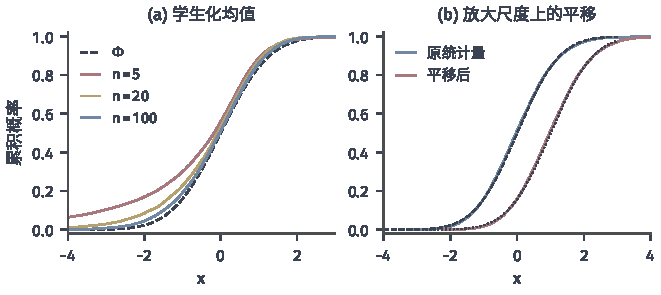
\includegraphics[width=112mm]{figures/02-abstract-mathematics/02-probability-spaces/matplotlib/wlim-studentized-shift/figure.pdf}
  \caption{随机标准化与尺度下的平移。总体为率参数$1$的指数分布，固定随机种子，每条曲线基于$20000$次重复。(a) 学生化均值$\sqrt n(\bar X_n-1)/S_n$的经验分布函数，$n=5,20,100$，虚线为$\Phi$。(b) $n=100$时$\sqrt n(\bar X_n-1)$（蓝）与把$\bar X_n$平移$1/\sqrt n=0.1$后的$\sqrt n(\bar X_n+1/\sqrt n-1)$（红）的经验分布函数，虚线与点线分别为$\Phi(x)$与$\Phi(x-1)$。}
  \label{fig:wlim-studentized-shift}
\end{figure}

\subsection{近似替换与渐近等价}

\paragraph{逐行可比较的近似量}
实际计算中常把一个统计量换成更容易处理的近似量，例如用分母$n$代替$n-1$，或删去一个高阶小项。替换是否改变分布极限，取决于两者的差是否依概率趋于零。

\begin{theorem}[近似替换]
\label{thm:wlim-approximation}
设对每个$n$，$\mathbb R^d$值的$\bm X_n$与$\widetilde{\bm X}_n$定义在同一概率空间上。若$\bm X_n\Rightarrow\bm X$，且$\lVert\widetilde{\bm X}_n-\bm X_n\rVert\to0$依概率成立，则$\widetilde{\bm X}_n\Rightarrow\bm X$。
\end{theorem}

\begin{proof}
写$\widetilde{\bm X}_n=\bm X_n+(\widetilde{\bm X}_n-\bm X_n)$，第二项依概率趋于常向量$\bm 0$，由Slutsky规则第一条即得。
\end{proof}

满足定理条件的两列称为渐近等价。一个易于检验的特例是$\mathbb P(\widetilde{\bm X}_n\neq\bm X_n)\to0$，因为$\mathbb P(\lVert\widetilde{\bm X}_n-\bm X_n\rVert>\varepsilon)\leq\mathbb P(\widetilde{\bm X}_n\neq\bm X_n)$。
定理的前提是二者能逐行比较。若只知道$\bm X_n$与$\widetilde{\bm X}_n$各自的分布，差$\widetilde{\bm X}_n-\bm X_n$连定义都没有，替换无从谈起。

\paragraph{缩放尺度下的误差}
替换条件必须在实际使用的尺度上检验。设$a_n>0$是确定的缩放系数，$\theta$是固定中心，已知$a_n(T_n-\theta)\Rightarrow L$。要用$\widetilde T_n$替换$T_n$，应验证
\[
  a_n(\widetilde T_n-T_n)\to0\quad\text{依概率成立},
\]
这时$a_n(\widetilde T_n-\theta)=a_n(T_n-\theta)+a_n(\widetilde T_n-T_n)\Rightarrow L$。仅有$\widetilde T_n-T_n\to0$不够。

最简单的反例是确定的平移。令$\widetilde T_n=T_n+1/\sqrt n$，差$1/\sqrt n$在原尺度上趋于零；但在$\sqrt n$尺度上，$\sqrt n(\widetilde T_n-T_n)=1$恒成立，极限整体平移一个单位。
图~\ref{fig:wlim-studentized-shift}(b)以$n=100$的指数样本均值为例：原尺度上的平移只有$0.1$，放大后的两条经验分布函数却分别贴近$\Phi(x)$与$\Phi(x-1)$。
统计模型中估计量的具体误差展开与Delta方法，在\BookPartRef{part:inference-and-causal-identification}{卷四“推断与因果识别”部分}展开；这里只保留通用的替换规则。

\section{标准化部分和的分布极限}
\label{sec:wlim-clt}

第~\ref{chap:random-variable-convergence}章研究了独立部分和是否收敛、样本平均是否靠近期望。本节研究另一个问题：把部分和中心化，再按它的波动尺度缩放，所得分布是否有稳定的极限。
我们按求和项满足的条件依次处理独立同分布、独立非同分布和随机向量三种情形。证明都使用第~\ref{sec:wlim-characteristic}节的特征函数，随机标准化与线性变换使用第~\ref{sec:wlim-joint-transform}节的规则。

\subsection{独立同分布情形}

\paragraph{特征函数的乘积极限}
标准化和的特征函数是$n$个相同因子的乘积。要比较两个乘积，下面的估计把乘积之差化成因子之差的和。

\begin{lemma}[乘积之差]
\label{lem:wlim-product-difference}
设复数$z_1,\ldots,z_n$与$w_1,\ldots,w_n$的模都不超过$1$，则
\[
  \Bigl|\prod_{k=1}^nz_k-\prod_{k=1}^nw_k\Bigr|\leq\sum_{k=1}^n|z_k-w_k|.
\]
\end{lemma}

\begin{proof}
对$n$归纳。$n=1$时显然成立。由
\[
  \prod_{k\leq n}z_k-\prod_{k\leq n}w_k=z_n\Bigl(\prod_{k<n}z_k-\prod_{k<n}w_k\Bigr)+(z_n-w_n)\prod_{k<n}w_k,
\]
以及$|z_n|\leq1$、$|\prod_{k<n}w_k|\leq1$，由归纳假设即得。
\end{proof}

\begin{theorem}[独立同分布的\term{中心极限定理}]
\label{thm:wlim-clt-iid}
设$X_1,X_2,\ldots$独立同分布，$\mathbb E X_1=\mu$，$0<\sigma^2=\operatorname{Var}X_1<\infty$。令
\[
  T_n=\frac{\sum_{k=1}^nX_k-n\mu}{\sigma\sqrt n}.
\]
则$T_n\Rightarrow N(0,1)$。
\end{theorem}

\begin{proof}
令$Y_k=(X_k-\mu)/\sigma$，它们独立同分布，均值为$0$，方差为$1$，$T_n=\sum_kY_k/\sqrt n$。由定理~\ref{thm:wlim-chf-operations}，
\[
  \varphi_{T_n}(t)=\Bigl[\varphi_{Y_1}\Bigl(\frac t{\sqrt n}\Bigr)\Bigr]^n.
\]
固定$t$。当$n\geq t^2/2$时$0\leq1-t^2/(2n)\leq1$，对$z_k=\varphi_{Y_1}(t/\sqrt n)$、$w_k=1-t^2/(2n)$用引理~\ref{lem:wlim-product-difference}，
\[
  \Bigl|\varphi_{T_n}(t)-\Bigl(1-\frac{t^2}{2n}\Bigr)^n\Bigr|\leq n\Bigl|\varphi_{Y_1}\Bigl(\frac t{\sqrt n}\Bigr)-1+\frac{t^2}{2n}\Bigr|.
\]
由定理~\ref{thm:wlim-chf-second-order}，$\varphi_{Y_1}(u)-1+u^2/2=o(u^2)$，取$u=t/\sqrt n$，右端是$n\cdot o(t^2/n)\to0$。又$(1-t^2/(2n))^n\to e^{-t^2/2}$，所以$\varphi_{T_n}(t)\to e^{-t^2/2}$。
极限是$N(0,1)$的特征函数（式~\eqref{eq:wlim-normal-chf}），在原点连续，由L\'evy连续性定理得$T_n\Rightarrow N(0,1)$。
\end{proof}

证明只用到有限二阶矩。条件$\sigma^2>0$不能省：若$\sigma^2=0$，各项几乎必然等于$\mu$，中心化部分和恒为零，含$1/\sigma$的标准化公式没有意义。

图~\ref{fig:wlim-clt-convergence}以指数总体为例检查定理。$n$个率参数为$1$的指数变量之和服从Gamma分布，$T_n$的分布函数可以精确计算。
(a)中$n=1$的分布函数在$-1$以下为零，形状明显偏斜；$n=16$与$n=64$时已经接近$\Phi$。(c)对应证明本身：特征函数$[\varphi_{Y_1}(t/\sqrt n)]^n$的实部随$n$增大贴近$e^{-t^2/2}$。

(b)记录分布函数的最大偏差$\sup_x|\mathbb P(T_n\leq x)-\Phi(x)|$：指数总体从$n=1$时的$0.159$降到$n=1000$时的$0.0042$，Bernoulli$(0.2)$总体从$0.49$降到$0.019$。两条点列在双对数坐标中都近似平行于斜率$-1/2$的参考线；Bernoulli总体的偏差更大，因为它是格点分布，分布函数始终有跳跃。
这些是对两个具体总体的观察。中心极限定理本身只断言偏差趋于零，不给出任何固定$n$下的误差界；讨论近似速度需要附加矩条件和专门的误差定理。

\begin{figure*}[htbp]
  \centering
  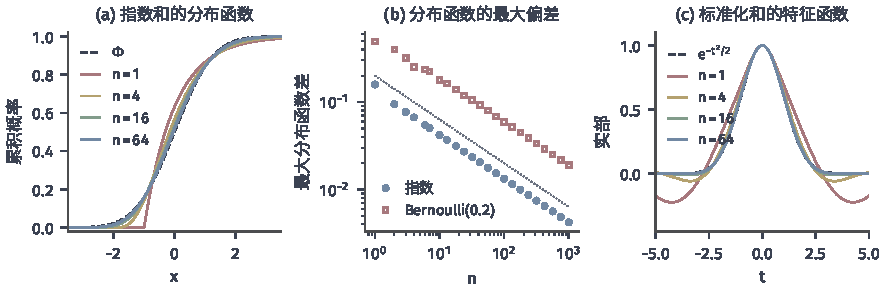
\includegraphics[width=150mm]{figures/02-abstract-mathematics/02-probability-spaces/matplotlib/wlim-clt-convergence/figure.pdf}
  \caption{标准化和向标准正态分布收敛。(a) 率参数$1$的指数总体，$T_n=(S_n-n)/\sqrt n$的精确分布函数（$S_n$服从形状$n$、率$1$的Gamma分布），$n=1,4,16,64$，虚线为$\Phi$。(b) 指数总体与$\operatorname{Bernoulli}(0.2)$总体的最大分布函数偏差，双对数坐标，点线为参考线$0.2/\sqrt n$。(c) 指数总体中心化后$\varphi_{Y_1}(u)=e^{-iu}/(1-iu)$，标准化和的特征函数$[\varphi_{Y_1}(t/\sqrt n)]^n$的实部与$e^{-t^2/2}$（虚线）。}
  \label{fig:wlim-clt-convergence}
\end{figure*}

\paragraph{样本平均的误差分布}
由连续映射$x\mapsto\sigma x$，定理~\ref{thm:wlim-clt-iid}等价于
\begin{equation}
  \sqrt n(\bar X_n-\mu)\Rightarrow N(0,\sigma^2).
  \label{eq:wlim-clt-mean}
\end{equation}
它与强大数定律（定理~\ref{thm:conv-slln}）回答不同的问题。大数定律说明$\bar X_n$几乎必然趋于$\mu$，即平均值最终停在哪里；式~\eqref{eq:wlim-clt-mean}把误差$\bar X_n-\mu$放大$\sqrt n$倍，说明放大后的波动具有什么形状。前者是同一概率空间上的逐样本结论，后者只涉及分布。

\BookChapterRef{chap:sampling-errors}{卷一“抽样分布与估计误差”章}陈述了中心极限定理并用它构造正态近似；本节在一般有限方差条件下给出了证明。
用样本标准差$S_n$替换$\sigma$时，例~\ref{ex:wlim-studentized-mean}已经说明，只需$S_n\to\sigma$依概率成立，再由Slutsky规则得到$\sqrt n(\bar X_n-\mu)/S_n\Rightarrow N(0,1)$，不需要分子与分母独立。

\subsection{独立非同分布情形}

\paragraph{三角阵与Lindeberg条件}
许多误差由不同来源、不同权重的项累加而成，例如加权平均$\sum_kw_k\varepsilon_k$中权重随样本量重新分配。这时求和项不再同分布，甚至每一行的项都随$n$改变。
我们把它们写成三角阵：对每个$n$，$X_{n,1},\ldots,X_{n,m_n}$同一行内相互独立，均值为零，方差有限，记
\[
  s_n^2=\sum_{k=1}^{m_n}\mathbb E X_{n,k}^2\in(0,\infty),\qquad T_n=\frac1{s_n}\sum_{k=1}^{m_n}X_{n,k}.
\]
均值不为零的项要先中心化。同一行内要求独立，不同行之间不作任何要求，各行甚至可以定义在不同的概率空间上。

\begin{definition}[\term{Lindeberg条件}]
\label{def:wlim-lindeberg-condition}
称上述三角阵满足Lindeberg条件，若对每个$\varepsilon>0$，
\[
  L_n(\varepsilon)=\frac1{s_n^2}\sum_{k=1}^{m_n}\mathbb E\bigl[X_{n,k}^2\,\mathbb I_{\{|X_{n,k}|>\varepsilon s_n\}}\bigr]\to0.
\]
\end{definition}

\begin{theorem}[Lindeberg中心极限定理]
\label{thm:wlim-lindeberg}
设三角阵$X_{n,k}$每行独立、均值为零、$s_n^2\in(0,\infty)$，并满足Lindeberg条件，则$T_n\Rightarrow N(0,1)$。
\end{theorem}

\paragraph{条件的含义}
$L_n(\varepsilon)$度量的是超出整体波动尺度$\varepsilon s_n$的那部分取值对总方差的贡献。条件要求这部分贡献在总方差中的比例趋于零，即和中没有哪一项能以不可忽略的方差份额单独产生大偏差。
由此还能推出每一项的方差占比一致趋于零：把$\mathbb E X_{n,k}^2$拆成$|X_{n,k}|\leq\varepsilon s_n$与$|X_{n,k}|>\varepsilon s_n$两部分，前者不超过$\varepsilon^2s_n^2$，于是
\begin{equation}
  \max_k\frac{\mathbb E X_{n,k}^2}{s_n^2}\leq\varepsilon^2+L_n(\varepsilon),
  \label{eq:wlim-max-share}
\end{equation}
先令$n\to\infty$，再令$\varepsilon\to0$，得最大方差占比趋于零。

独立同分布情形是特例：取$X_{n,k}=X_k-\mu$、$m_n=n$，则$s_n^2=n\sigma^2$，
\[
  L_n(\varepsilon)=\frac1{\sigma^2}\mathbb E\bigl[(X_1-\mu)^2\,\mathbb I_{\{|X_1-\mu|>\varepsilon\sigma\sqrt n\}}\bigr]\to0,
\]
因为被积函数逐点趋于零且以可积的$(X_1-\mu)^2$为界。

\paragraph{Lindeberg定理的证明}
证明沿用同分布情形的路线，只是每个因子不同，需要把小偏差与大偏差分开估计。

\begin{proof}[定理~\ref{thm:wlim-lindeberg}的证明]
记$Y_{n,k}=X_{n,k}/s_n$、$\sigma_{n,k}^2=\mathbb E Y_{n,k}^2$，则$\sum_k\sigma_{n,k}^2=1$，由式~\eqref{eq:wlim-max-share}有$\max_k\sigma_{n,k}^2\to0$。固定$t$，由行内独立，$\varphi_{T_n}(t)=\prod_k\varphi_{Y_{n,k}}(t)$。

第一步，与二次近似比较。由引理~\ref{lem:wlim-exp-remainder}，在$\{|Y_{n,k}|\leq\varepsilon\}$上用三阶界，在其补集上用二阶界：
\[
  \begin{aligned}
  \Bigl|\varphi_{Y_{n,k}}(t)-1+\frac{t^2\sigma_{n,k}^2}2\Bigr|
  &\leq\frac{|t|^3}6\mathbb E\bigl[|Y_{n,k}|^3\mathbb I_{\{|Y_{n,k}|\leq\varepsilon\}}\bigr]+t^2\,\mathbb E\bigl[Y_{n,k}^2\mathbb I_{\{|Y_{n,k}|>\varepsilon\}}\bigr]\\
  &\leq\frac{|t|^3\varepsilon}6\sigma_{n,k}^2+t^2\,\mathbb E\bigl[Y_{n,k}^2\mathbb I_{\{|Y_{n,k}|>\varepsilon\}}\bigr].
  \end{aligned}
\]
对$k$求和，右端之和不超过$|t|^3\varepsilon/6+t^2L_n(\varepsilon)$。当$n$充分大时$t^2\max_k\sigma_{n,k}^2\leq2$，各个$1-t^2\sigma_{n,k}^2/2$落在$[0,1]$中，由引理~\ref{lem:wlim-product-difference}，
\[
  \limsup_n\Bigl|\varphi_{T_n}(t)-\prod_k\Bigl(1-\frac{t^2\sigma_{n,k}^2}2\Bigr)\Bigr|\leq\frac{|t|^3\varepsilon}6,
\]
$\varepsilon$任意，所以左端极限为零。

第二步，与正态特征函数比较。记$x_k=t^2\sigma_{n,k}^2/2\geq0$，则$\prod_ke^{-x_k}=e^{-t^2/2}$。对$x\geq0$有$|e^{-x}-1+x|\leq x^2/2$，再用一次引理~\ref{lem:wlim-product-difference}，
\[
  \Bigl|\prod_k(1-x_k)-e^{-t^2/2}\Bigr|\leq\sum_k\frac{x_k^2}2\leq\frac12\Bigl(\max_kx_k\Bigr)\sum_kx_k=\frac{t^4}8\max_k\sigma_{n,k}^2\to0.
\]
两步合并得$\varphi_{T_n}(t)\to e^{-t^2/2}$，由L\'evy连续性定理即得结论。
\end{proof}

证明中Lindeberg条件起两个作用：在第一步直接控制大偏差项的二阶余项；经式~\eqref{eq:wlim-max-share}保证最大方差占比趋于零，使第一步的各个$1-t^2\sigma_{n,k}^2/2$落在$[0,1]$中，并使第二步的误差消失。小偏差项用三阶估计，但三阶矩只在$\{|Y_{n,k}|\leq\varepsilon\}$上出现，自然有界，所以定理不需要三阶矩。

\paragraph{Lyapunov条件与不等权误差}
Lindeberg条件需要计算截断二阶矩。较易检验的是下面的高阶矩条件：存在$\delta>0$使
\[
  \frac1{s_n^{2+\delta}}\sum_{k=1}^{m_n}\mathbb E|X_{n,k}|^{2+\delta}\to0,
\]
称为\term{Lyapunov条件}。在$\{|X_{n,k}|>\varepsilon s_n\}$上，$X_{n,k}^2\leq|X_{n,k}|^{2+\delta}/(\varepsilon s_n)^\delta$，逐项求和得$L_n(\varepsilon)\leq\varepsilon^{-\delta}s_n^{-2-\delta}\sum_k\mathbb E|X_{n,k}|^{2+\delta}\to0$，所以Lyapunov条件推出Lindeberg条件。
注意条件是一个比值的极限，“各项都有$2+\delta$阶矩”本身并不够。

\begin{example}[不等权的独立误差]
\label{ex:wlim-unequal-weights}
设$R_1,R_2,\ldots$独立，以相等概率取$\pm1$。
第一种方案取$X_{n,k}=kR_k$，$1\leq k\leq n$，即第$k$个误差的权重为$k$。此时$s_n^2=\sum_{k\leq n}k^2=n(n+1)(2n+1)/6$，最大方差占比$n^2/s_n^2\approx3/n\to0$。由于$|X_{n,k}|\leq n$而$s_n\geq n^{3/2}/\sqrt3$，当$n>3/\varepsilon^2$时没有任何项超过$\varepsilon s_n$，$L_n(\varepsilon)=0$；Lindeberg条件成立，$T_n\Rightarrow N(0,1)$。
第二种方案让首项主导：$X_{n,1}=2\sqrt{n-1}\,R_1$，$X_{n,k}=R_k$（$2\leq k\leq n$）。此时$s_n^2=5(n-1)$，首项的方差占比恒为$4/5$；当$\varepsilon<2/\sqrt5$时首项总超过$\varepsilon s_n$，$L_n(\varepsilon)\geq4/5$，Lindeberg条件不成立。
事实上$T_n=\bigl(2R_1+\sum_{k\geq2}R_k/\sqrt{n-1}\bigr)/\sqrt5$。由定理~\ref{thm:wlim-clt-iid}，括号中的第二项依分布收敛到$N(0,1)$，且它与$R_1$在同一行内独立；由定理~\ref{thm:wlim-independent-product}与连续映射，$T_n\Rightarrow(2R+G)/\sqrt5$，其中$R$与$G\sim N(0,1)$独立。这一极限方差为$1$，却是$N(\pm2/\sqrt5,1/5)$的等权混合，不是正态分布。
\end{example}

图~\ref{fig:wlim-lindeberg-triangular}对照两种方案。(a)中递增权重方案的最大方差占比按$3/n$的量级下降，主导首项方案停在$4/5$。(b)中$n=200$时，前者的行和直方图贴合标准正态密度，后者呈现以$\pm2/\sqrt5\approx\pm0.89$为中心的双峰，与混合正态密度一致。
三角阵的用途正在于此：权重和参与求和的项随$n$变化时，必须对每一行重新计算总方差和各项的相对贡献，而不能沿用同分布情形的结论。
在最大方差占比趋于零的前提下，Lindeberg条件也是正态极限的必要条件（Feller定理），本章不证明这一方向。

\begin{figure}[htbp]
  \centering
  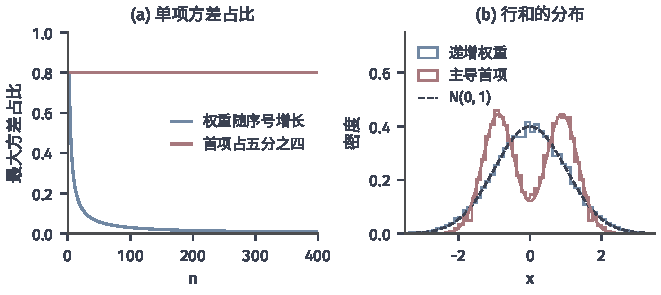
\includegraphics[width=112mm]{figures/02-abstract-mathematics/02-probability-spaces/matplotlib/wlim-lindeberg-triangular/figure.pdf}
  \caption{三角阵中单项方差占比与行和的分布，$R_k$为独立的Rademacher变量。(a) 最大方差占比$\max_k\mathbb E X_{n,k}^2/s_n^2$：权重$X_{n,k}=kR_k$时为$6n/((n+1)(2n+1))$；首项$X_{n,1}=2\sqrt{n-1}R_1$主导时恒为$4/5$。(b) $n=200$时两种方案的行和$T_n$的直方图（固定随机种子，$20000$次重复），虚线为$N(0,1)$密度，红色实线为主导首项方案的极限密度，即$N(\pm2/\sqrt5,1/5)$的等权混合。}
  \label{fig:wlim-lindeberg-triangular}
\end{figure}

\subsection{随机向量情形}

\paragraph{逐方向的标量极限}
许多统计量同时包含几个样本平均，例如样本均值与样本二阶矩，我们需要它们的联合误差分布。Cram\'er--Wold判据把这个问题化为每个方向上的一维中心极限定理。

\begin{theorem}[多维中心极限定理]
\label{thm:wlim-clt-vector}
设$\bm X_1,\bm X_2,\ldots$是独立同分布的$\mathbb R^d$值随机向量，均值为$\bm\mu$，协方差矩阵$\bm\Sigma$有限。则
\[
  \sqrt n(\bar{\bm X}_n-\bm\mu)\Rightarrow N(\bm 0,\bm\Sigma).
\]
\end{theorem}

\begin{proof}
固定$\bm a\in\mathbb R^d$。单项投影$\bm a^\top(\bm X_k-\bm\mu)$独立同分布，均值为零，方差为$\bm a^\top\bm\Sigma\bm a$。
若$\bm a^\top\bm\Sigma\bm a>0$，由定理~\ref{thm:wlim-clt-iid}与式~\eqref{eq:wlim-clt-mean}，$\bm a^\top\sqrt n(\bar{\bm X}_n-\bm\mu)\Rightarrow N(0,\bm a^\top\bm\Sigma\bm a)$。
若$\bm a^\top\bm\Sigma\bm a=0$，各项投影几乎必然为零，$\bm a^\top\sqrt n(\bar{\bm X}_n-\bm\mu)=0$几乎必然成立，同样收敛到$N(0,0)=\delta_0$。
另一方面，若$\bm W\sim N(\bm 0,\bm\Sigma)$，由式~\eqref{eq:wlim-mvn-chf}，$\varphi_{\bm a^\top\bm W}(s)=\varphi_{\bm W}(s\bm a)=e^{-s^2\bm a^\top\bm\Sigma\bm a/2}$，所以$\bm a^\top\bm W\sim N(0,\bm a^\top\bm\Sigma\bm a)$。由Cram\'er--Wold判据即得结论。
\end{proof}

\paragraph{奇异协方差与线性变换}
定理只要求$\bm\Sigma$半正定，不要求可逆，因而不依赖于白化或密度。$\bm\Sigma$奇异时，存在方向$\bm a\neq\bm 0$使$\bm a^\top\bm\Sigma\bm a=0$，极限分布集中在与这些方向正交的低维子空间上。
对固定的$m\times d$矩阵$\bm B$，由连续映射定理与式~\eqref{eq:wlim-mvn-chf}，
\[
  \bm B\sqrt n(\bar{\bm X}_n-\bm\mu)\Rightarrow N(\bm 0,\bm B\bm\Sigma\bm B^\top),
\]
所以联合极限同时给出任意有限个线性组合的联合波动。

图~\ref{fig:wlim-clt-vector}以$\xi\sim$率参数$1$的指数分布为例。(a)取$\bm X=(\xi,\xi^2)$，均值$(1,2)$，由$\mathbb E\xi^3=6$、$\mathbb E\xi^4=24$得
\[
  \bm\Sigma=\begin{pmatrix}1&4\\4&20\end{pmatrix};
\]
$n=200$时$1500$个$\sqrt n(\bar{\bm X}_n-\bm\mu)$的散点沿$\bm\Sigma$的主轴方向伸展，与$N(\bm 0,\bm\Sigma)$的$95\%$概率椭圆相符，样本协方差约为$\begin{pmatrix}1.01&4.13\\4.13&20.8\end{pmatrix}$。
(b)给出两个方向的投影：$\bm a=(1,0)$的极限方差为$1$，$\bm a=(1,-0.2)$的极限方差为$1-1.6+0.8=0.2$，直方图分别贴合相应的正态密度。后一个方向几乎与长轴垂直，波动远小于任一坐标，这正是只看坐标无法得到的信息。
(c)取$\bm X=(\xi,3-2\xi)$，$\bm\Sigma=\begin{pmatrix}1&-2\\-2&4\end{pmatrix}$的秩为一，方向$\bm a=(2,1)$上的方差为零，所有散点都落在直线$V_2=-2V_1$上；极限$N(\bm 0,\bm\Sigma)$集中在同一条直线上，没有二维密度。

\begin{figure*}[htbp]
  \centering
  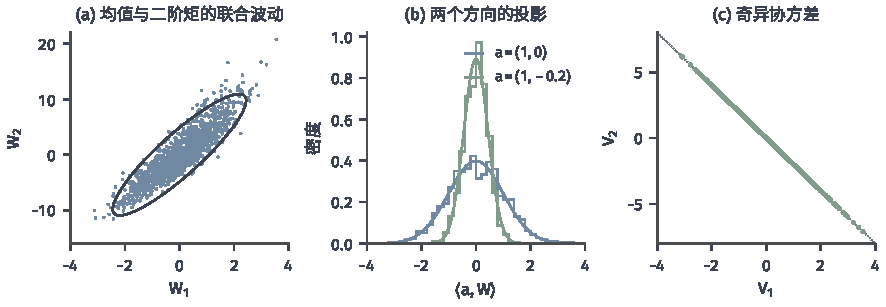
\includegraphics[width=150mm]{figures/02-abstract-mathematics/02-probability-spaces/matplotlib/wlim-clt-vector/figure.pdf}
  \caption{二维中心极限定理，$\xi$服从率参数$1$的指数分布，$n=200$，固定随机种子，$1500$次重复。(a) $\bm W=\sqrt n(\bar{\bm X}_n-\bm\mu)$，$\bm X=(\xi,\xi^2)$，实线为$N(\bm 0,\bm\Sigma)$的$95\%$概率椭圆，$\bm\Sigma=\bigl(\begin{smallmatrix}1&4\\4&20\end{smallmatrix}\bigr)$。(b) $\bm W$沿$\bm a=(1,0)$与$\bm a=(1,-0.2)$的投影直方图，实线为极限密度$N(0,1)$与$N(0,0.2)$。(c) $\bm X=(\xi,3-2\xi)$时的$\bm V=\sqrt n(\bar{\bm X}_n-\bm\mu)$，协方差矩阵秩为一，点全部落在直线$V_2=-2V_1$（点线）上。}
  \label{fig:wlim-clt-vector}
\end{figure*}

这里的维数$d$固定，结论属于有限维分布理论。把部分和看成随时间变化的整条路径，并研究路径的分布极限，需要路径空间上的紧性，留给\BookPartRef{part:dynamical-systems-control-decision-and-games}{卷三“过程与轨迹演化”部分}。

\section{本章小结}
\label{sec:wlim-summary}

章首的模拟研究中，不同样本量的数据分别生成，只能比较分布。本章的回答是：$T_n$的分布趋近$N(0,1)$，意思是每个有界连续函数的平均值都收敛，在实轴上等价于分布函数在极限的连续点处收敛。
由此能直接读出边界零质量事件的概率极限；闭集与开集只有单向不等式；均值、矩等无界积分还需要一致可积这一尾部条件，尖峰分布说明弱收敛本身不控制它。弱收敛只记录分布，不记录配对，所以它推不出依概率收敛，极限为常数时才是例外。

本章区分了围绕分布列的四类任务。给定候选极限时检验收敛，用测试函数或Portmanteau判据；没有候选极限时取得子列，靠一致紧性与Prokhorov定理；识别子列极限，靠特征函数的唯一性与L\'evy连续性定理；对几个随机量作运算，先由Cram\'er--Wold判据、行内独立或与常数配对得到联合极限，再用连续映射、Slutsky规则与近似替换传递极限。
各个条件分管不同的风险：一致紧性防止质量逃到紧集之外，一致可积防止无界积分的尾部贡献，事件边界、映射不连续点与随机分母的零点各有自己的零测条件，不能用一种控制代替其余。

回到独立部分和，第~\ref{chap:random-variable-convergence}章的大数定律说明样本平均最终停在期望处，本章的中心极限定理刻画误差放大$\sqrt n$倍后的形状。
证明的核心是特征函数把独立和变成乘积，有限二阶矩给出二阶展开，乘积极限给出$e^{-t^2/2}$。Lindeberg条件把这一论证推广到每行内部独立、权重各异的三角阵，它要求没有哪一项占据不可忽略的方差份额；向量情形则由逐方向的一维结论与Cram\'er--Wold判据合成，协方差矩阵可以奇异。
这些结论都只涉及固定维数的分布，不提供有限样本误差界。比较分布的更强距离、估计量的渐近推断与整条随机路径的极限，分别在后续相应部分展开。
